\documentclass[a4, 10pt]{cmspaper}

%\usepackage{multirow}
%\usepackage{subfigure}
%\usepackage{subfig}

\usepackage[pdftex]{graphicx}
\usepackage{verbatim}
\usepackage{amsmath}
\usepackage{epsfig}
\usepackage{array}% in the preamble

\newcommand{\be}{\begin{equation}}
\newcommand{\ee}{\end{equation}}
\newcommand{\bea}{\begin{eqnarray}}
\newcommand{\eea}{\end{eqnarray}}
\newcommand{\nn}{\nonumber}
\newcommand{\dsn}{\displaystyle{\not}}

\begin{document}

%==============================================================================
% title page for few authors

\begin{titlepage}

% select one of the following and type in the proper number:
%  \internalnote{2009/000}
%  \conferencereport{2005/000}
   \date{\today}

 \title{Performance of QCD background estimation methods for single lepton SUSY searches}

 \begin{Authlist}
   O.~Buchmueller\Aref{a}, Z.~Hatherell\Aref{a}, G.~Karapostoli\Aref{a}, A.~Sparrow\Aref{a}, P.~Sphicas\Aref{b,c},
	A.~Tapper\Aref{a}
       \Instfoot{ic}{a) Imperial College London, United Kingdom}	
     \Instfoot{cern}{b) CERN, Geneva, Switzerland}	
\Instfoot{uoa}{c) University of Athens, Greece}
   \end{Authlist}

\begin{abstract}
The performance of data-driven QCD background estimation methods to be used for single lepton SUSY searches is studied. The methods are contructed using Monte Carlo datasets, and the performance is studied with an X $pb^{-1}$ sample of 7 TeV LHC collisions. The data provides many events with one electron and at least one jet, with which we validate the method of predicting the disibution of the $\alpha_{T}$ jet-balancing kinematic variable. This is undertaken by inverting the cuts on $\Delta \phi$ and $\Delta \eta$ Electron ID variables. Another method utilises Isolation templates in control regions to predict the distribution in the signal region. 
\end{abstract}


\end{titlepage}

\tableofcontents
\newpage
\setcounter{page}{2}
\section{Introduction}
\label{sec:intro}

We present a study of two methods for predicting the QCD background contribution to the search for SUSY using a signature of one (and only one) electron plus jets.

The first method employs the Isolation distribution and its description in terms of two components, one from the combination of hadronic jets and heavy-flavor ($c,b$) jets and one from photon conversions. The background due to hadronic jets is modeled using a control sample formed using an anti-selection on the $\Delta \phi$ and $\Delta \eta$ matching cuts.  The background due to photon conversions is modeled using a control sample formed using explicitly reconstructed conversions.  We then demonstrate that the two control samples can be used to predict successfully the backgrounds remaining after a tight electron selection.  

The second method utilizes the kinematic $\alpha_{T}$ jet-balancing method which has been recently developed within CMS, as a generic approach to discover New Physics (most favorably supersymmetry) in the single-lepton plus missing energy channel. It is possible to extend the $\alpha_{T}$ method from the all-hadronic channels, in order to reduce the QCD background and gain reliable control over severe jet mismeasurements.  In this note we use the anti-selection Control Sample to obtain a description of the background due to QCD processes and demonstrate that the estimated value and shape of the background agrees quite well with the actual value and shape from the Monte Carlo.

The methods are then ``commissioned'' with CMS data in the context of the first 1pb$^{-1}$ of pp collisions at a center-of-mass energy of 7 TeV.

\section{Analysis Framework}
\label{sec:framework}

The coding structure used for this analysis has been developed in CMSSW\_3\_6\_1 releases on top of the SusyAnalysis software package \cite{susypat1}, which is itself an extension of the Physics Analysis Toolkit (PAT) \cite{susypat2}. A detailed description of the code can be found here \cite{susypat}. The PAT provides post-processing of reconstructed event data, in order to eliminate the information and condense the number of physics objects in an event for simplified physics analysis purposes. The framework comprises three layers. The initial layer reprocesses RECO or AOD data with the aim to refine the reconstructed object collections (remove duplicates for example).

The second layer formulates the cleaned data into simple object collections, such as PAT::Jet, PAT::Electron, PAT::Muon etc. which are sorted in uncorrected transverse energy.  At this stage, the data are available for use in analysis. A third layer may optionally used as well, providing utilities such as cross cleaning between various object collections. %The purpose of the cross-cleaning module is to eliminate overlaps between physics objects which share energy deposits, such as jets and electrons, and correct their energy appropriately. 
The output of the above PAT processing steps is a ROOT ntuple which is further analysed with private code as described here \cite{ICNT}.

\section{Monte Carlo and Data samples}

The analysis uses QCD Monte Carlo data samples for QCD background processes as well as the W + jets process -for studying signal contamination effects-, produced with the Summer09 simulation production for Physics at 7~TeV \cite{data}, with CMS. The Standard Model QCD background processes considered are listed below:
\begin{itemize}
\item QCD EM enriched in complete bins exclusive of $\hat{p_{T}}$  ([20,30],[30,80],[80,170]) were produced with the event generator Pythia6.
%. MadGraph is a matrix-element event generator, where higher order effects, like the emission of extra ISR gluons, are included in the matrix-element calculation\footnote{This is opposed to parton-shower based generators, like PYTHIA, where the emission of extra jets, other than the ones emitted by the $2 \rightarrow 2$ hard scattering process, is simulated by the parton-shower model.}.
\item QCD BC$\rightarrow e$ also in complete exclusive bins of  $\hat{p_{T}}$  ([20,30],[30,80],[80,170]) produced by Pythia6.
\item QCD Jets in inclusive bin of $\hat{p_{T}}$ $>$ 30~GeV and 80~GeV, produced with the event generator Pythia6. These samples are exceptionally used in the Isolation template method next. 
\item $W \rightarrow e\nu$ sample  simulated by Pythia6.
\end{itemize}

The numbers of events available in these datasets as well as the equivalent integrated luminosity they correspond to, are detailed in Table \ref{tab:datasets}. The luminosity figures give an indication of the statistics used in the study, although next the resulting plots have been normalized to 1pb$^{-1}$ of integrated luminosity, unless stated otherwise.

\begin{table}[h!]
\begin{center}
\begin{tabular}{|c|c|c|c|}
\hline
Data Set & N events & $\sigma$ (pb) & Equivalent luminosity (pb$^{-1}$)\\
\hline
QCD BCtoE [20$<\hat{p_{T}}<$30]& 1100000  & 108330 & 10.15\\
QCD BCtoE [30$<\hat{p_{T}}<$80] & 1000000 & 138762 & 7.21\\
QCD BCtoE [80$<\hat{p_{T}}<$170 & 1208000 & 9422.4 & 128.21\\
\hline
QCD EM Enriched [20$<\hat{p_{T}}<$30] & 9714886 & 1719150 & 5.65\\
QCD EM Enriched [30$<\hat{p_{T}}<$80] & 9683936 & 3498700 & 2.77\\
QCD EM Enriched [80$<\hat{p_{T}}<$170] & 5494911 & 134088 & 40.98\\
\hline
QCDJets $\hat{p_{T}}>$170 & 3171950 & 25470 & 124.54\\
\hline
W + jets & 10034822 & 17830 & 415.18\\
\hline
\end{tabular}
\end{center}
\caption{\textit{The Monte Carlo datasets used to investigate the Delta ID Inversion method in QCD backgrounds. The available Lumniosity is shown, although plots produced are normalised to 1pb$^{-1}$ for the purpose of understanding the near-term reach of CMS.}}
\label{tab:datasets}
\end{table}

The background estimation methods to be presented are finally commissioned using the following Data~\cite{PDWG} and Monte Carlo (for direct data-MC comparisons) samples: 
\begin{itemize}
\item 7 TeV data: 
\begin{itemize}
\item JetMETTau Secondary Dataset (SD)
\begin{verbatim}
/JetMETTau/Run2010A-PromptReco-v1/RECO 
/JetMETTau/Run2010A-PromptReco-v2/RECO
/MinimumBias/Commissioning10-SD_JetMETTau-v9/RECO 
\end{verbatim}
\item EG SD
\begin{verbatim}
/EG/Run2010A-PromptReco-v1/RECO 
/EG/Run2010A-PromptReco-v2/RECO 
/MinimumBias/Commissioning10-SD_EG-v9/RECO
\end{verbatim}

\end{itemize}
\item 7 TeV Monte Carlo: \begin{verbatim}/QCD_Pt-15_7TeV-pythia8/Spring10-START3X_V26B-v1/GEN-SIM-RECO \end{verbatim}
\end{itemize}




%\newpage
\section{Event selection}
\label{sec:evtsel}

\subsection{Pre-selection for single electron analysis}
%A single-electron event for searches with $\alpha_{T}$ is defined through a series of requirements on basic physics objects. 
The current analysis follows a series of requirements on the basic physics objects to define events with 1-electron in the final state. The baseline selection is:
\begin{itemize}
\item The High Level Trigger (HLT) requirement is HLT\_Jet15U, which is currently the lowest threshold unprescaled trigger. %HLT\_Ele15\_SW\_L1R.
\item Exactly one electron of the following definition:
\begin{itemize}
\item Reconstructed with the PixelMatchGsfElectron algorithm.
\item $p_{T} >$ 10 GeV, 20 GeV\footnote{The Analysis is targeting to commission the background estimation methods for electron $P_{T}$ threshold at 10 GeV; however, a 20 GeV threshold is always checked to allow synchronization with the Egamma POG recommendations and EWK PAG analyses of CMS.  }
\item $|\eta| <2.4$
\item Passes the Cut Based ID formed by simple, yet robust, variables (these are the $H/E$, the super-cluster (SC) - track matching variables $\Delta \phi$,$\Delta \eta$, and shower shape variable $\sigma_{i\eta i\eta}$ and the combined relative Isolation\footnote{The cut based ID selection cuts are chosen to correspond to an 80\% efficiency in the $W\rightarrow e\nu$ analysis.}). 
\end{itemize}
\item The event is vetoed if there are any muons of the following definition:
\begin{itemize}
\item $p_{T} >$ 15 GeV
\item $|\eta| <2.1$
\item Passes ID requirement: GlobalMuon
\end{itemize}
\item Jets are reconstructed with ak5jet algorithm run on standard Calorimeter Jets.  The jet selection is as follows:
\begin{itemize}
\item $p_{T} >$ 20 GeV (corrected energy)
\item $|\eta| <5$
\item EMF $<$0.9 (in the MC only); a jet can be further rejected if it is found close to a tight and isolated electron within $\Delta R$=0.3 and the ratio of electron to jet energy is $p_{T}(e)/p_{T}(jet) > 0.7$. 
\item in real data, in order to reject noise from the calorimeters, jets are furthermore required to pass \textit{loose jet ID} (identification) criteria which are summarised as:
\begin{itemize}
\item  $|\eta| > 2.6$ or EMF $>0.01$
\item  fHPD (fraction of energy contributed by the highest hybrid photo-diode readout in the HCAL) $< 0.98$
\item  n90Hits (number of RecHits contributing 90\% of the jet energy) $> 1$
 \end{itemize}
\end{itemize}

\end{itemize}

According to the standard recommendations for a global \textit{event cleaning} when running on the Data, the following requirements have been imposed as well: 
\begin{itemize}
\item L1 technical trigger bit 0 is active: to ensure consistent timing with LHC bunch crossing.
\item HLT PhysicsDeclared bit is ON; which indicates that all CMS systems were operational with stable beams in the accelerator.
\item At least one good vertex (excluding fake) with number of degrees of freedom, $N_{\text{dof}}>=5$, and vertex position along the beam direction of $|z_{\text{vtx}}| < 15$~cm. 
\item Remove events with many fake tracks (also known as monster events) by requiring the ratio of HighPurity tracks over the total number of tracks to be greater than 25\% in events that have 10 or more tracks.
\end{itemize}

\subsection{Simple Cut-Based Electron Selection}
\label{sec:EID}
Efficient electron selection is important in physics analyses with electron final states to enhance the selection of signal. This is especially crucial when the $E_{T}$ threshold is low, as is characteristic of many SUSY searches, as the background and fake rate increase. In the era of LHC start-up, it is essential to use simple and robust variables.

The electron selection used in this study follows the recommendations of the e-gamma group\cite{elsel}. Simple cuts are made on a small number of robust variables suitable for early data taking at the LHC. Different cuts are applied to electrons in the ECAL barrel to those in the ECAL endcap. Aside from this no categorisation is applied. 

The Electron Selection  variables can be described in three groups: 
\begin{itemize}
\item Typical electron ID variables ( $\sigma_{i\eta i\eta}$, $\Delta \phi$, $\Delta \eta$ and H/E).
\begin{itemize}
\item $\sigma_{i\eta, i\eta}$ measures the RMS shower width in the eta direction.
\item $\Delta \phi_{\textrm{in}}$ and $\Delta \eta_{\textrm{in}}$ give the geometric match, in $\phi$ and $\eta$ respectively between the GSF track trajectory and the ECAL supercluster.
\item Tracker, ECAL and HCAL isolation formed respectively from the sume of ECAL RecHits, HCAL RecHits and track $p_{\textrm{T}}$ in a cone of $\Delta R < 0.4$. The centre of the cone is taken to be the supercluster for the calorimeter isolations and the track direction at the vertex for the tracker.
\item $H/E$ is the ratio of the energy deposited in the HCAL behind the electron seed to the energy of the supercluster.

\end{itemize}
\item Isolation variables (Tracker Isolation, HCAL Isolation and ECAL Isolation)
\item Conversion Rejection Tools; photon conversions are rejected initially by requiring that the track associated to the electron has a hit in the first pixel layer pf tracker pixels. Additional rejection power against converted photons is achieved by using the variables described here~\cite{conv}.
\end{itemize}

We apply this electron selection with values at a working point corresponding to 80\% efficiency for the W$\rightarrow e$ analysis. One of the advantages of this new cut based selection is thiat it allows the inversion of one or more of the variables, a common tool in background-subtraction and signal extraction methods.




%\clearpage

\section{QCD Background Estimation Methods}

\label{sec:QCD_bkgd_est}

In the context of a search for SUSY using a signature containing an electron, there are three sources of ``background electrons'', namely ``non-prompt'' electrons:
\begin{enumerate}
\item Jets which are either mismeasured or have very atypical hadronization, yielding ``electrons'' which pass the basic identification and selection requirements.  We refer to these as ``Jet electrons'' (Jet-e) in what follows.
\item Photon conversions in the tracker material.  We refer to these as ``Conversion electrons'' (Conv-e) in what follows.
\item Electrons from semileptonic decays of $c$ and $b-$ flavored hadrons.  We refer to these as ``Heavy Flavor electrons'' (HF-e) in what follows.
\end{enumerate}

There are numerous methods for estimating both the amount of background and the shape of this background as a function of various variables (the transverse momentum, pseudorapidity, and in some cases more complicated topological variables) that remains in a data sample after a specific set of selection cuts.  All these methods employ ``control samples'' which are selected via appropriate alternate requirements which do not affect the shape of the variable in question (e.g. the transverse momentum of the lepton).  As an example, we mention the well-known ``Isolation inversion'' method, where one uses events failing the isolation requirement and an extrapolation into the ``selection region'', i.e. where events pass the isolation requirement, to estimate the amount of background in the latter~\cite{cornel}.  A crucial issue in most methods is the demonstration that the extrapolation from the ``control region'' to the ``selection region'' is correct or, at least, its deficiencies are small and can be estimated reliably.  There are two elements that enter this extrapolation from a control region to a selection region in the case of electrons:
\begin{itemize}
\item The actual knowledge of the full dependence of any single source of background electrons on the variable in question.  As an example, concentrating on only the Jet-e background, there remains the issue of how to obtain reliably the full shape of the isolation of the Jet-e background which passes all selection cuts from some other ``control sample'' which passes a slightly different set of cuts.
\item The presence of the three different sources of background implies that each of these backgrounds may well exhibit a different dependence on the variable in question.  As an example, the isolation distribution from Jet-e and Conv-e need not be (and is in fact not) the same.  This implies that it may be necessary to determine explicitly the amount of each background in the selection region, and to then form the total expected background as the sum of the three individual components.
\end{itemize}
For the sake of concreteness, in what follows we will refer to the ``Isolation variable'', even though the discussion applies equally well to essentially most variables.

Of the two above issues, the first is usually tackled initially using Monte Carlo: one uses generator-level information to obtain the Isolation distribution for any specific background (e.g. Jet-e) and then compares this shape with that extracted from the ``control sample''.  Assuming that this comparison is favorable, i.e. that the shape from the control sample can adequately describe the shape in the selection sample, the next and final step is to compare this shape with the one extracted from data using the ``control selection''. 

Tackling the second issue is more complicated though. First, the presence of three sources of background (instead of two) implies more degrees of freedom in the fitting (and in general in describing) any particular variable -- e.g. the Isolation variable. Second, the relative amount of each source needs to be determined for the final selection sample.

In this section, we concentrate on the following three key observations to address all of the above:
\begin{enumerate}
\item A good method for identifying a control sample for the Jet-e background is the reversal of the matching cuts $\Delta\eta$ and $\Delta\phi$.  These two variables exhibit near independence from other selection variables, especially the isolation variable
\item The isolation distributions of the Jet-e and HF-e backgrounds seem to be similar and to be collectively described well by the same control sample (via the matching-cut reversal).
\item A fairly pure sample of Conv-e background can be identified using the existing conversion-identification tools. This sample can then be used to extract a template for other variables in question, e.g. the Isolation distribution or the $\alpha_T$ distribution.
\end{enumerate}
In what follows, we exploit these three observations to obtain the shapes of the total background in both the isolation and $\alpha_T$ distributions.  Moreover, a fit to the isolation distribution using different shapes (templates) for the Jet-e and Conv-e backgrounds yields an estimate of the absolute number of background events in the selection region.

\subsection{Modeling the electron backgrounds}
\label{sec:modeling}

In what follows, we will consider more closely two different definitions of ``Isolation'', namely ``Calo Isolation'', which is defined using only the sum of the energies in the ECAL and HCAL, and ``Combined Isolation'' which includes also the transverse momenta of charged-particles tracks around the electron.  Since the search for SUSY may necessitate using low-$P_T$ leptons, we investigate the behavior for two different thresholds of 10 and 20 GeV on the electron $P_T$.

The isolation distribution using only calorimeter isolation is displayed in Figure~\ref{fig:caloIso_MC}, whereas the combined (relative) isolation is shown in Figure~\ref{fig:combIso_MC}.  It can be seen that two backgrounds, namely the Jet-e and JF-e have distributions which are fairly similar for both the Calo-Iso and Comb-Iso.
\begin{figure}[htb!]
\centering
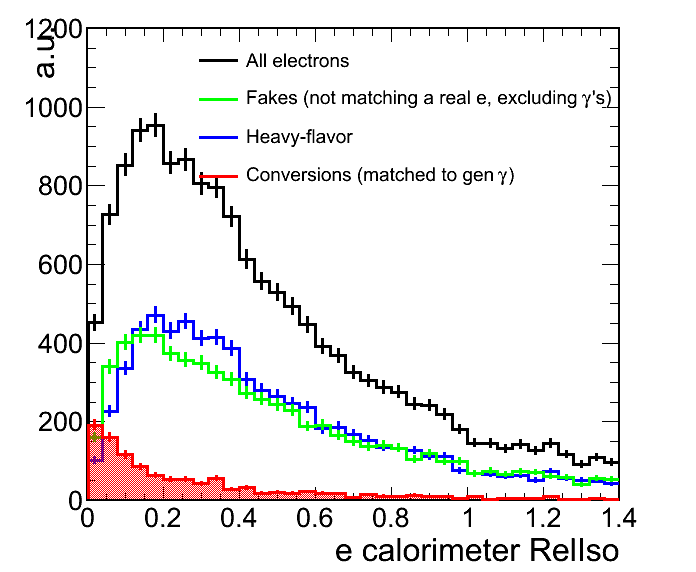
\includegraphics[scale=0.32]{Plots/caloIso_pt10_MC.png}
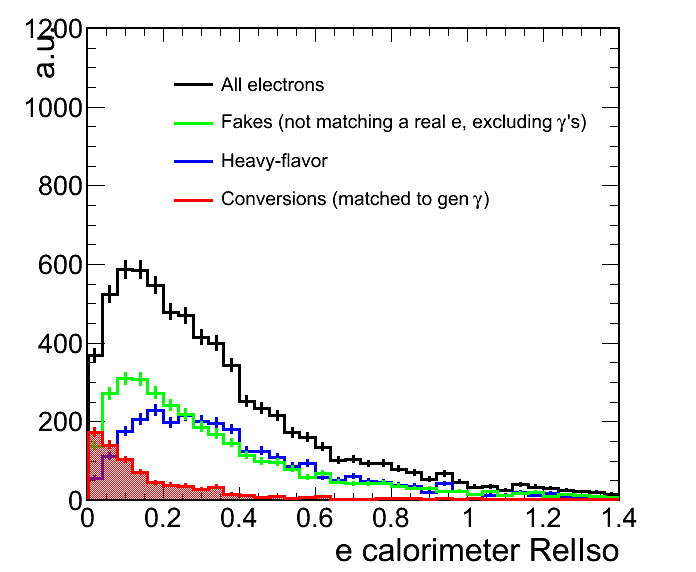
\includegraphics[scale=0.32]{Plots/caloIso_pt20_MC.png}
\caption{\textit{The Calorimeter Isolation distribution from Monte Carlo simulation (QCD pythia $\hat{p}_{T} > 80$).  On the left for a threshold of 10 GeV on the electron and the right for a 20 GeV threshold.  The three sources of background, namely Jet-e, HF-e and Conv-e are shown separately, along with the sum of the three.}}\label{fig:caloIso_MC}
\end{figure}

\begin{figure}[h!]
\centering
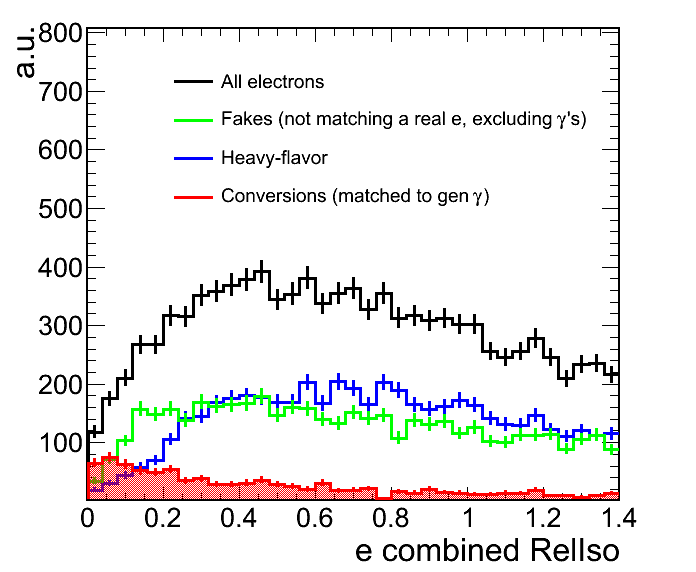
\includegraphics[scale=0.32]{Plots/combIso_pt10_MC.png}
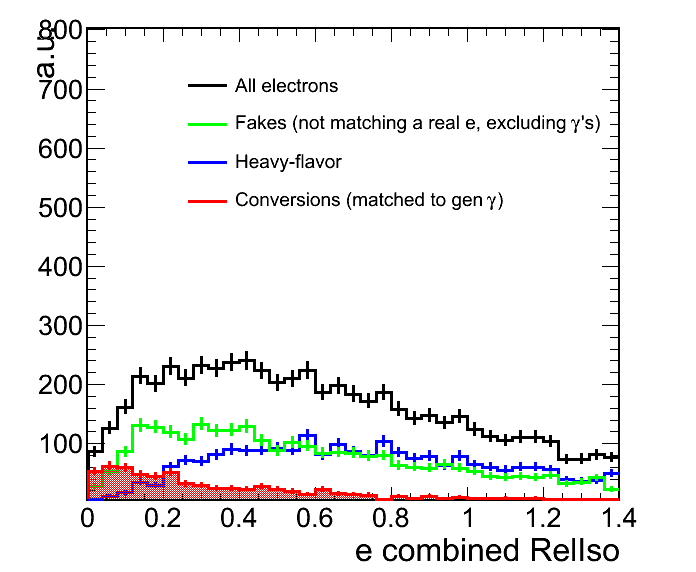
\includegraphics[scale=0.32]{Plots/combIso_pt20_MC.png}
\caption{\textit{The Combined Isolation distribution from Monte Carlo simulation  (QCD pythia $\hat{p}_{T} > 80$).  On the left for a threshold of 10 GeV on the electron and the right for a 20 GeV threshold.  The three sources of background, namely Jet-e, HF-e and Conv-e are shown separately, along with the sum of the three.}}\label{fig:combIso_MC}
\end{figure}

%\clearpage

\subsubsection{Isolation Distribution for the Jet-e and HF-e backgrounds}

The first step is to define a control sample for the combination of Jet-e and HF-e and to see how well it can describe the Isolation distributions (both CaloIso and CombIso) in the selection region.  As stated previously, this is done by inverting the $\Delta \eta$(trk-SC) and $\Delta \phi$ (trk-SC) id cuts in the electron selection. The selected events in this method pass the pre-selection described in Section~\ref{sec:evtsel}, while the anti-selected are those events which pass the selection with an electron that passes all selection criteria {\it except} the $\Delta \phi$ (trk-SC) and $\Delta \eta$(trk-SC) ones.  The resulting distributions are shown in Figure~\ref{fig:caloIso_fakes} for the CaloIso and in Figure~\ref{fig:combIso_fakes} for the CombIso.

\begin{figure}[ht!]
\centering
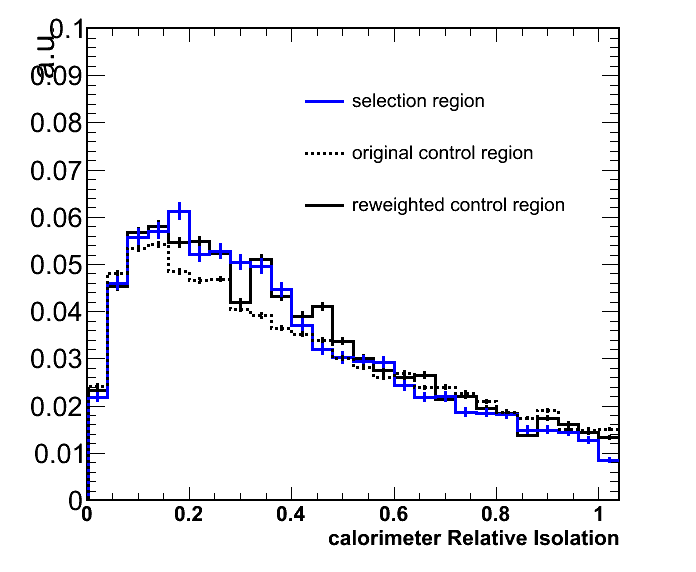
\includegraphics[scale=0.32]{Plots/caloIso_pt10_fakes.png}
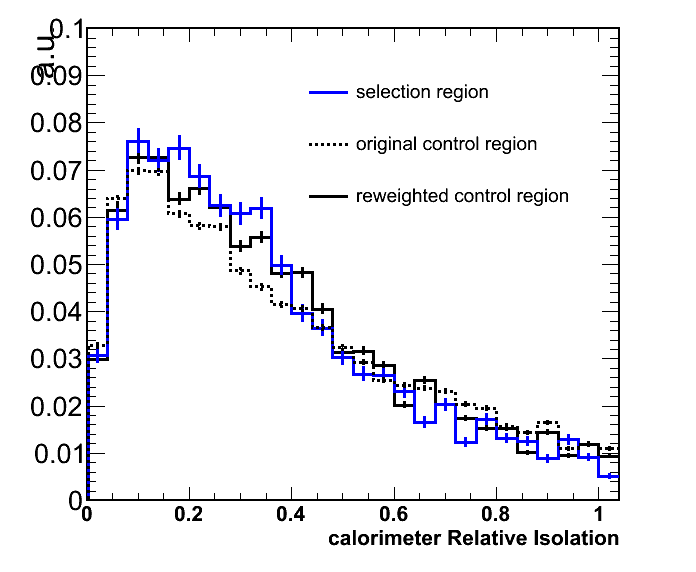
\includegraphics[scale=0.32]{Plots/caloIso_pt20_fakes.png}
\caption{\textit{The Calorimeter Isolation distribution from Monte Carlo simulation of the combined Jet-e+HF-e background.   On the left for a threshold of 10 GeV on the electron and the right for a 20 GeV threshold.  The solid blue line is the total Jet-e+HF-e background in the selection region, whereas the dashed line is the distribution from the control sample, defined via the anti-selection on the matching cuts.  The solid black line is the result of re-weighting the control sample for the jet spectra -- as described in the text.}}\label{fig:caloIso_fakes}
\end{figure}

\begin{figure}[h!]
\centering
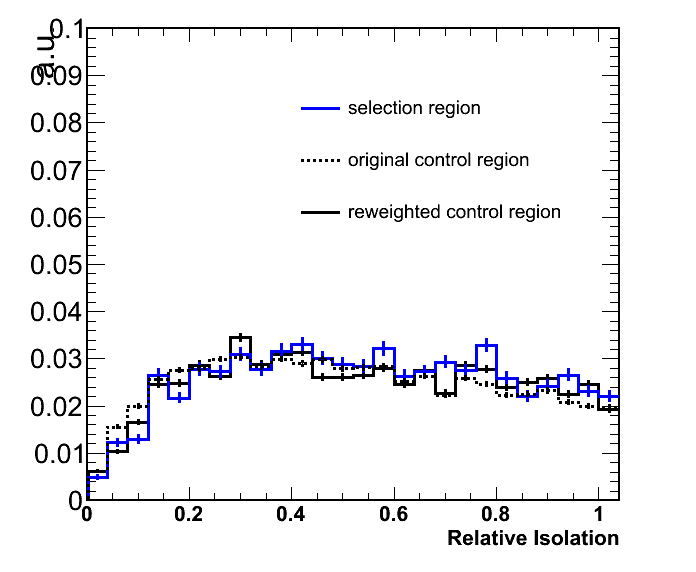
\includegraphics[scale=0.32]{Plots/combIso_pt10_fakes.png}
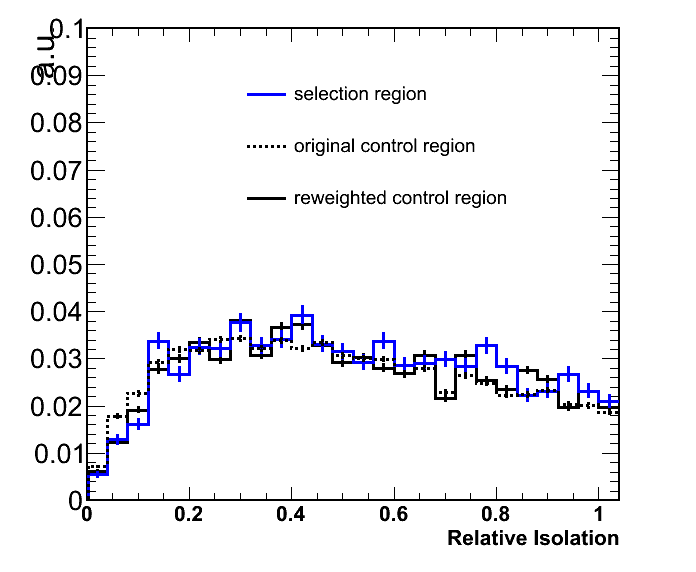
\includegraphics[scale=0.32]{Plots/combIso_pt20_fakes.png}
\caption{\textit{Same as Figure~\ref{fig:caloIso_fakes} only this time for the Combined Isolation distribution.}}\label{fig:combIso_fakes}
\end{figure}

It can be seen that the shape of the Combined Isolation distribution from the Control Region is quite similar to that of the distribution from the Selection Region -- a very encouraging result which indicates that the anti-selection of the matching cuts yields a good method for modeling non-conversion electrons. A closer look into various properties of these events, however, yields a slight difference in the Calorimeter Isolation distributions.  As can be seen in Figure~\ref{fig:caloIso_fakes}, for small values of the CaloIso variable the two distributions, i.e. from the Control and Selection regions have a small difference (around CaloIso$\approx 0.1-0.4$).  This is more easily seen in Figure~\ref{fig:ratio_control_fakesHF} where the ratio of the Calorimeter Isolation distributions from the Selection and Control regions is displayed. 

\begin{figure}[h!]
\centering
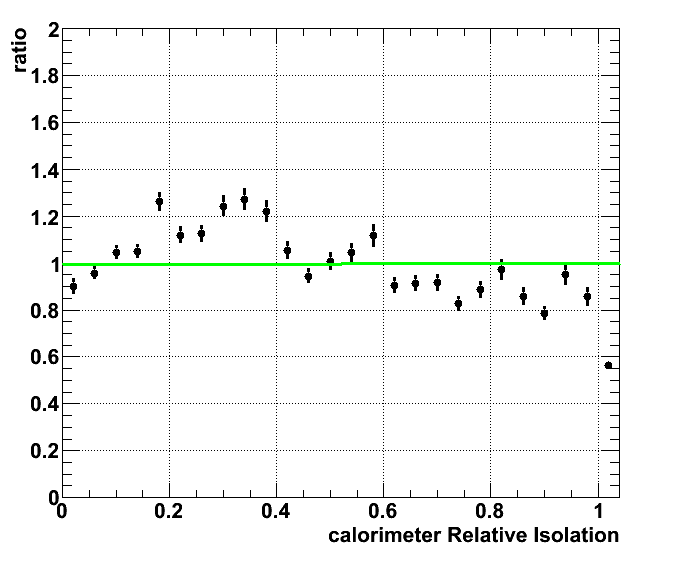
\includegraphics[scale=0.32]{Plots/ratio_control_fakesHF.png}
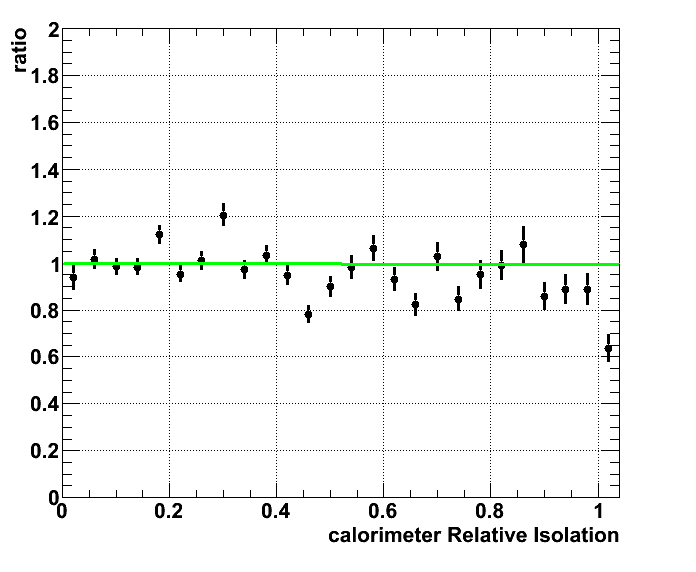
\includegraphics[scale=0.32]{Plots/ratio_re-control_fakesHF.png}
\caption{\textit{The ratio of the Calorimeter Isolation distributions from the Selection Region and the Control Region.  Left plot: the ratio of the two ``raw'' distributions (the dashed curves) seen in Figure~\ref{fig:caloIso_fakes}.  Right plot: {\it after} the re-weighting correction, i.e. the ratio of the two black lines in Figure~\ref{fig:caloIso_fakes}.}}\label{fig:ratio_control_fakesHF}
\end{figure}

We have investigated possible sources of this difference, from the surrounding objects, and in particular any jet that (possibly) accompanies the electron candidate.  There are small differences in the shapes of the associated jet $P_T$ spectrum as well as from the distance in $\eta-\phi$ space ($\Delta R$) between the jet and the electron.  These can be seen in Figure~\ref{fig:Pt-DR-comparison}.

\begin{figure}[h!]
\centering
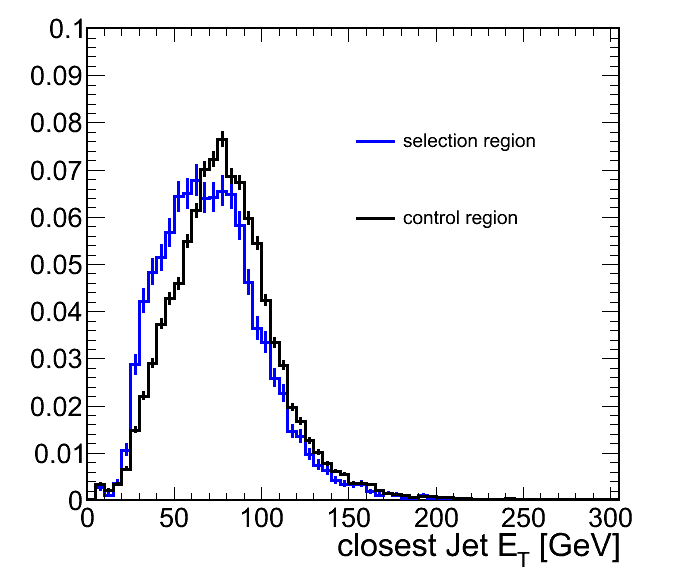
\includegraphics[scale=0.32]{Plots/jetEt_dependence.png}
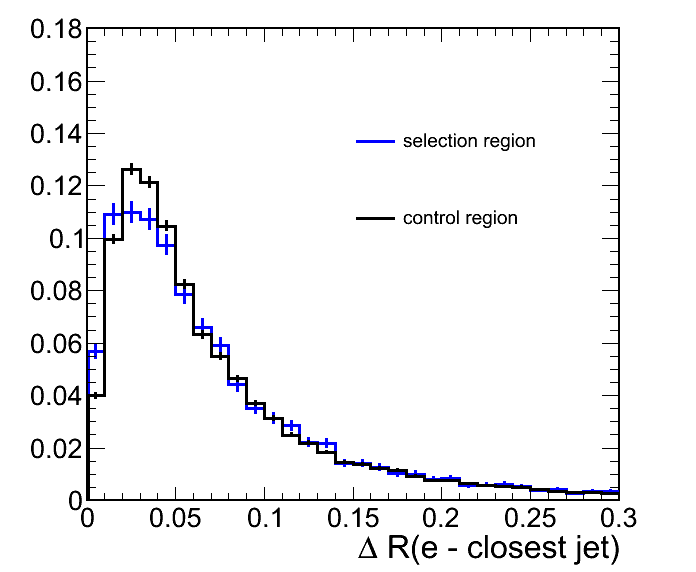
\includegraphics[scale=0.32]{Plots/dR_dependence.png}
\caption{\textit{Distributions of the transverse momentum ($P_T$) and distance to the electron $\Delta R$) of the nearest jet.}}\label{fig:Pt-DR-comparison}
\end{figure}

Presumably, these differences arise from a small correlation between the matching variables and the density of the overall hadronic energy surrounding or near the electron candidate.  Since the difference is small, we have attempted to correct the ``predicted'' shape, i.e. the shape from the Control Region, by applying a weight which depends on the associated Jet $P_T$ and the $\Delta R$ between the jet and the electron.  The solid blue line in \ref{fig:caloIso_fakes} is the result of this re-weighting.  It can be seen that the corrected Calorimeter Isolation distribution from the Control Region now describes the distribution from the Selection Region quite well.  This is more readily seen in Figure~\ref{fig:ratio_control_fakesHF} (right).

We have also applied the same correction to the Combined Isolation distribution, which did not exhibit a visible difference between the Control and Selection Regions, to ensure that the correction did not adversely affect this original agreement.  As can be seen in Figure~\ref{fig:combIso_fakes} the corrected distribution still describes the Selection Region very well.

\subsubsection{Isolation distribution from the Conv-e background}

Electrons from photon conversions are identified using the standard criteria of the Conversion Finder tools \cite{conv}. A suitable Control sample for modeling the Conv-e component in the Isolation distribution can be obtained by electrons that pass the Conversion tools (i.e. using an anti-veto on the Conversion rejection requirements). There are two algorithms to identify electrons from converted photons:

\begin{itemize} 
\item \textit{Missing expected hits}: the algorithm asks that there be $> 0$ expected layers with a missing hit before the first valid hit on the electron's track. The number of missing expected hits in front of the innermost valid hit is available via the electron's gsfTrack Hit Pattern.
\item \textit{Partner track finding}: the algorithm looks for the electron's partner track from a converted photon in the generalTrack collection. The track is identified as a conversion partner if: 
\begin{itemize}
\item the track has opposite charge to the electron track.
\item Approximately the same $\delta \cot(\theta)$ , in this case: $|\delta \cot(\theta)| < 0.02$.
\item small distance (dist) in the $r-\phi$ plane, in this case: $|\text{dist}| < 0.02$. 
\end{itemize}
\end{itemize}

The Conv-e component of the Isolation in the Selection region is formed using only electrons which match a generated photon at MC generator (``MC-truth'') level. The shape of this component is compared with the one obtained from the Conv-e control region as described previously.  The resulting distributions are shown in Figure~\ref{fig:caloIso_conv} for the CaloIso and in Figure~\ref{fig:combIso_conv} for the CombIso.  It can be seen that the shape of both distributions in the Selection Region is described well by the Control Region.

\begin{figure}[h!]
\centering
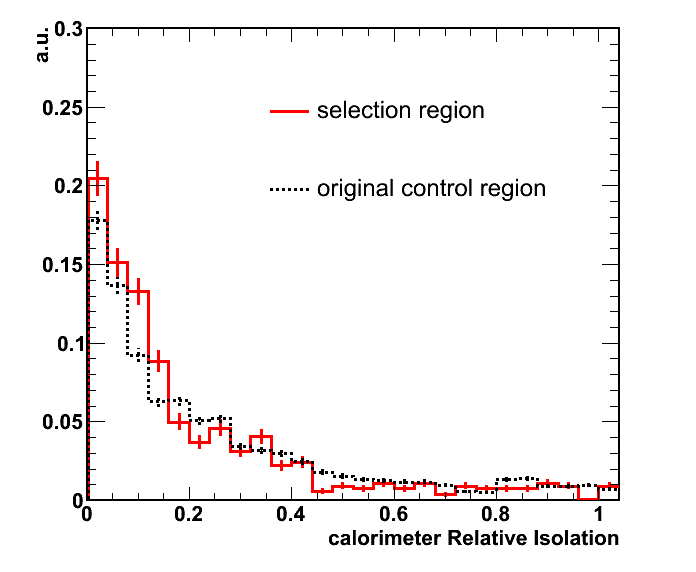
\includegraphics[scale=0.32]{Plots/caloIso_pt10_conv.png}
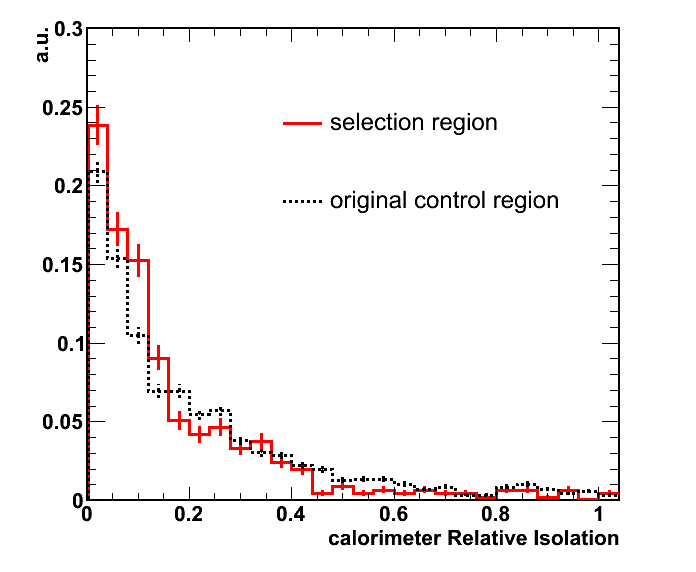
\includegraphics[scale=0.32]{Plots/caloIso_pt20_conv.png}
\caption{\textit{The Calorimeter Isolation distribution from Monte Carlo simulation of electrons from conversions.   On the left for a threshold of 10 GeV on the electron and the right for a 20 GeV threshold.  The solid red line is the Conv-e background in the selection region, whereas the dashed line is the distribution from the control sample, defined via the conversion identification requirements described in the text.}}\label{fig:caloIso_conv}
\end{figure}

\begin{figure}[h!]
\centering
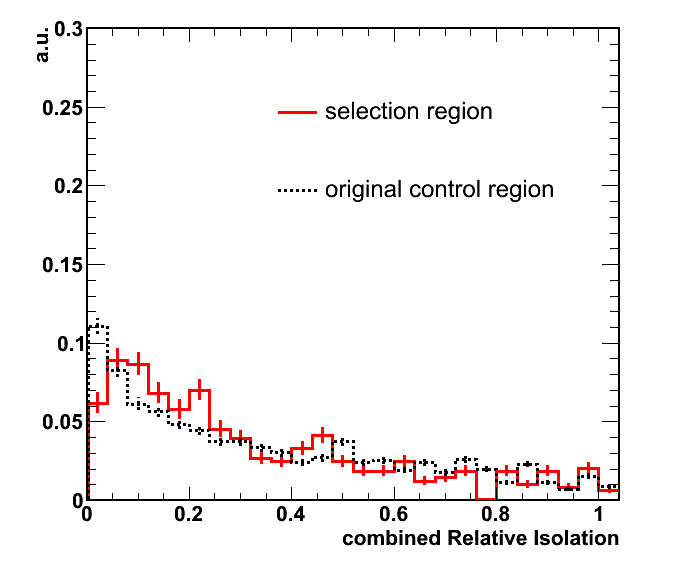
\includegraphics[scale=0.32]{Plots/combIso_pt10_conv.png}
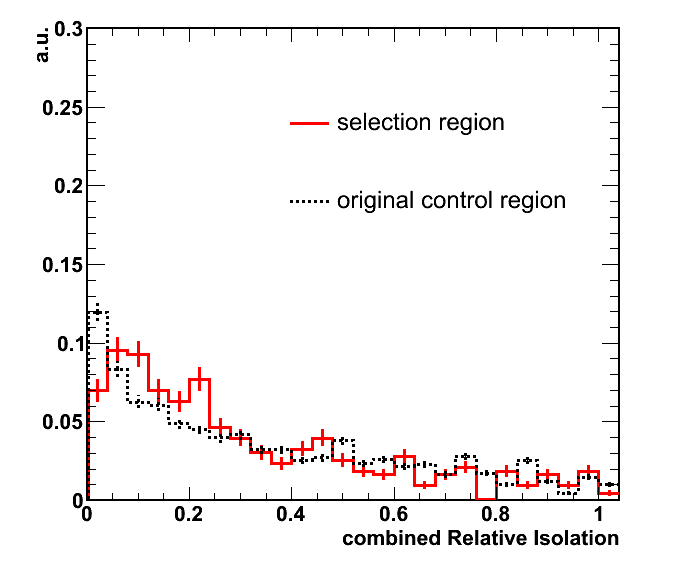
\includegraphics[scale=0.32]{Plots/combIso_pt20_conv.png}
\caption{\textit{Same as Figure~\ref{fig:caloIso_conv} only this time for the Combined Isolation distribution.}}\label{fig:combIso_conv}
\end{figure}

\subsubsection{Describing the Isolation distribution in the Selection Region}

Having demonstrated that two independent Control Samples can yield good descriptions of the Isolation distribution in the Selection Region for each background (i.e the combined Jet-e+HF-e and the Conv-e) we next attempt to describe the full Isolation distribution in the Selection Region as a sum of two components, with the template of each component extracted as described above: the combined Jet-e and HF-e background is described from the corrected (re-weighted) anti-selected (for matching) sample, whereas the Conv-e background is described from the sample passing the conversion-identification criteria.  We thus fit the total Isolation distribution using these two components, leaving the relative normalization of the two as a free fit parameter.  The result is shown in Figure~\ref{fig:caloIso_fit} for the calorimeter isolation and shows a very good description of the total background distribution.  It can also be observed that the conversion component becomes more relevant at high $P_T(e)$.  The corresponding distributions for the Combined Isolation variable are described equally well (see Figure~\ref{fig:combIso_fit}).
%  In the interest of saving space, and since previously it is the Calorimeter Isolation distribution which exhibited some differences, in what follows we will concentrate only on the Calorimeter Isolation (even though the corresponding Combined Isolation was always checked and found to be in excellent agreement).

\begin{figure}[h!]
\centering
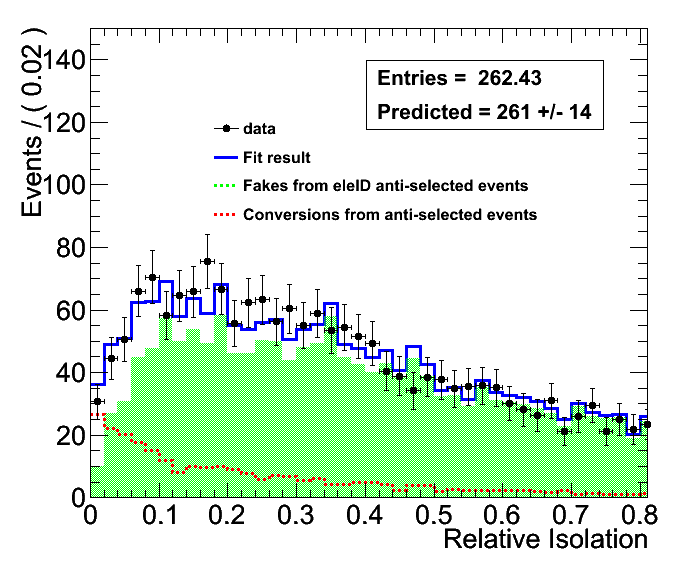
\includegraphics[scale=0.32]{Plots/caloIso_pt10_fit.png}
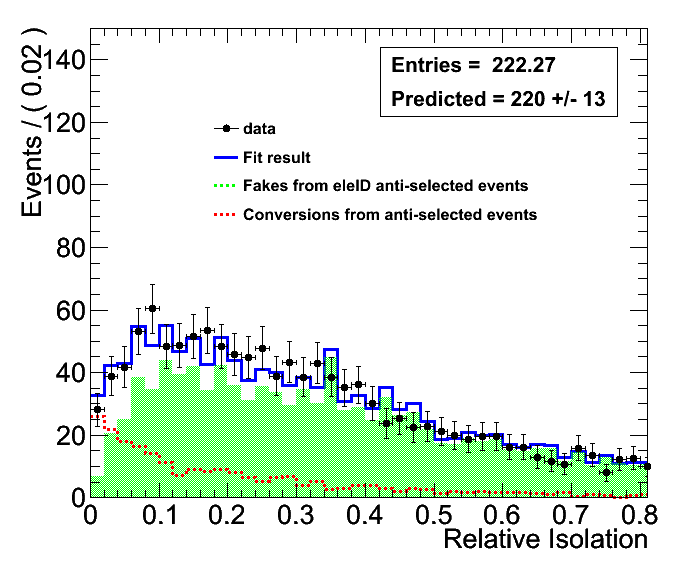
\includegraphics[scale=0.32]{Plots/caloIso_pt20_fit.png}
\caption{\textit{The Calorimeter Isolation distribution from Monte Carlo simulation of background electrons. On the left for a threshold of 10 GeV on the electron and the right for a 20 GeV threshold.  The dashed lines are the two background components as extracted from the two Control Samples, whereas the sum of the ``predicted'' background is the solid line.}}\label{fig:caloIso_fit}
\end{figure}

\begin{figure}[h!]
\centering
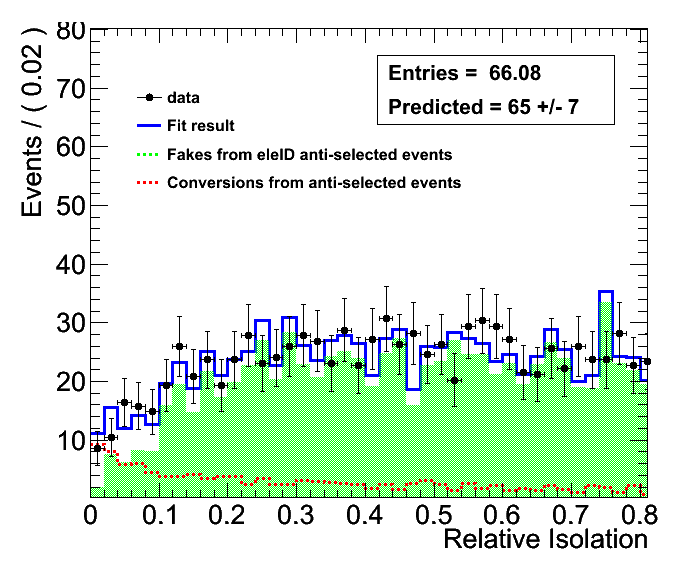
\includegraphics[scale=0.32]{Plots/combIso_pt10_fit.png}
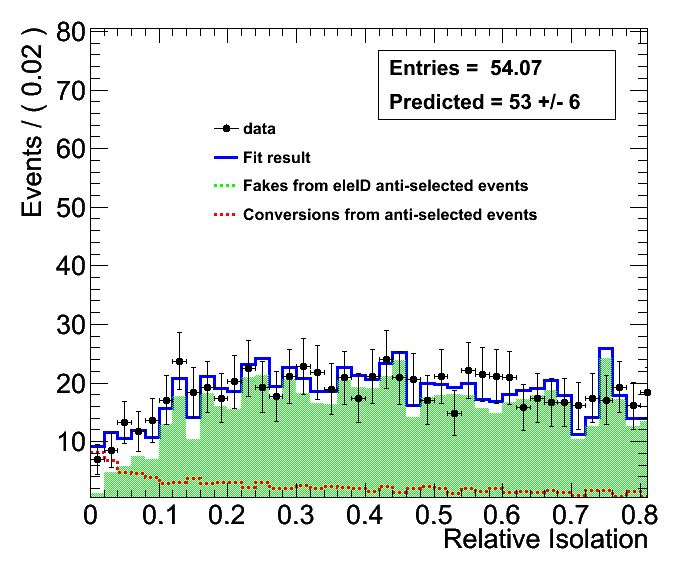
\includegraphics[scale=0.32]{Plots/combIso_pt20_fit.png}
\caption{\textit{The combined Isolation distribution from Monte Carlo simulation of background electrons. On the left for a threshold of 10 GeV on the electron and the right for a 20 GeV threshold.  The dashed lines are the two background components as extracted from the two Control Samples, whereas the sum of the ``predicted'' background is the solid line.}}\label{fig:combIso_fit}
\end{figure}

\subsubsection{Describing the Isolation distribution in the presence of prompt electrons}
\label{mc_wcontamin}

In the data, the Isolation distribution in the Selection region will also be populated by prompt electrons sources -in addition to QCD sources - with  $W \rightarrow e\nu$ being the most prominent one (and electrons from semi-leptonic $t\bar{t}$ events). We have thus investigated the performance of the Isolation template method in the presence of W events. In this case, one needs to add to the fit function a third component (template) to describe the Isolation shape for prompt electrons. We note here that an Isolation template for prompt electrons can be easily extracted using data-driven ways (e.g. the random cones technique) or even using a MC shape directly. 

The selection of electrons with offline $P_{T} > 10$ GeV implies that one needs to incorporate the low $\hat{p}_{T}$-bins of QCD MC samples. We therefore include both the QCD inclusive jets samples QCD\_pt30 and QCD\_pt80, with a weight normalized to $0.1 \text{pb}^{-1}$ of integrated luminosity\footnote{The luminosity chosen to normalize the QCD MC samples corresponds roughly to the available statistics of the QCD\_pt30 sample; so that QCD\_pt30 events are worked with a weight of $\approx 1$}. The W pythia sample is also normalized accordingly and included in the Selection. We finally repeat the Isolation template method, using the combined relative Isolation distribution, as previously described, in order to extract the number of fake (background) electron events that fall into the Signal Selection region (RelIso $<0.1$). Figure~\ref{fig:w_combIso_fit} (left) shows the combined fit for $P_{T}(e)>10 $ GeV in the presence of a W signal. The same fit is repeated on the right plot, where now a $\text{pfMET} < 20 $ GeV cut has been applied to the Selection, to suppress the $W \rightarrow e\nu$ component. The latter case descreases the error on the measurement due to smaller correlations in the fit parameters. 

Armed with this result, we next investigate the performance of the template method on fake electron events (in signal region RelIso $< 0.1$) in the presence of W events, and with increasing a cut on the hadronic activity in the event -namely applying successively an $H_{T}$ cut. Figure~\ref{fig:w_fitprediction_mc} shows a comparison of the number of background events observed in the signal region, in black, versus the number of fake electron events predicted in blue. Also superimposed are the number of total events, - including Ws -, in the signal region shown in red dots. A cut of $\text{pfMET} < 20$~GeV has been applied. Similar plots are repeated for electrons with $P_{T}> 20$ GeV (see Figures~\ref{fig:w_combIso_fit_pt20} and~\ref{fig:w_fitprediction_mc_pt20}).

%\clearpage

\begin{figure}[h!]
\centering
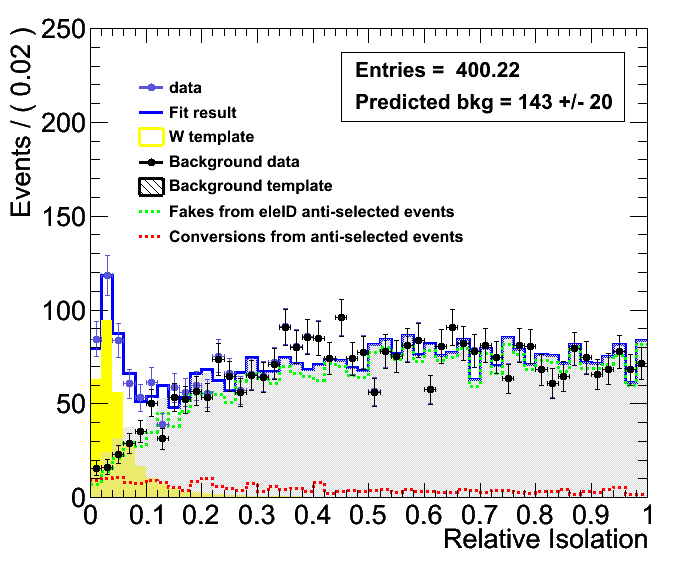
\includegraphics[scale=0.32]{Plots/w_combIso_pt10_fit_MC.png}
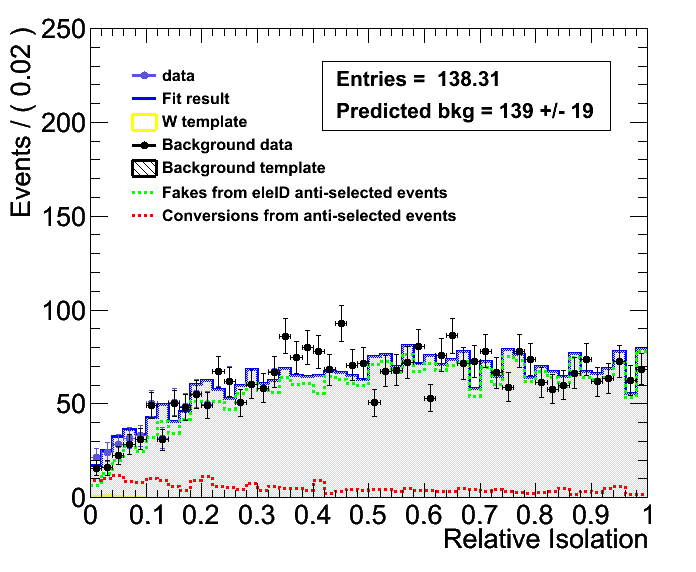
\includegraphics[scale=0.32]{Plots/w_combIso_pt10_METanticut_fit_MC.png}
\caption{\textit{The combined Isolation distribution from Monte Carlo simulation of background electrons - using the PYTHIA QCD\_pt30 and QCD\_pt80 samples -, and prompt electrons - using the PYTHIA $W \rightarrow e\nu$ sample, for $p_{T}(e)>$ 10 GeV. On the right plot, a pfMET $ < 20$~GeV anti-cut has been applied. The dashed lines are the two background components as extracted from the two Control Samples, whereas the total ``predicted'' background is the solid line.}}
\label{fig:w_combIso_fit}
\end{figure}

\begin{figure}[h!]
\centering
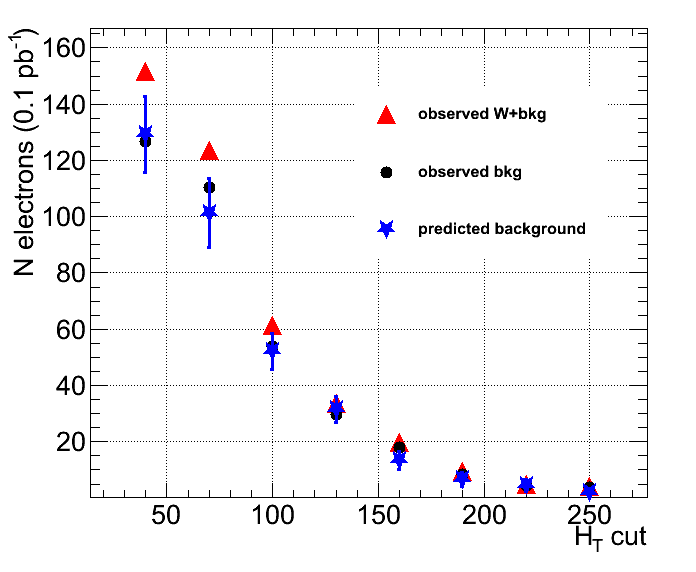
\includegraphics[width=80mm]{Plots/w_fitprediction_pt10_METanticut_vsHT_MC.png}
%\end{center}
\caption{\textit{The number of truth background electrons (in black dots) in signal region, RelIso $< 0.1$, are compared to the fit prediction (in blue stars), as a function of the cut in the hadronic activity of the event ($H_{T}$ cut). A cut of pfMET $<20$~GeV has been applied to suppress sources of prompt electrons (Ws here). The number of total truth electron events - including residual Ws - is also shown superimposed in red triangles. }}
\label{fig:w_fitprediction_mc}
\end{figure}

\begin{figure}[h!]
\centering
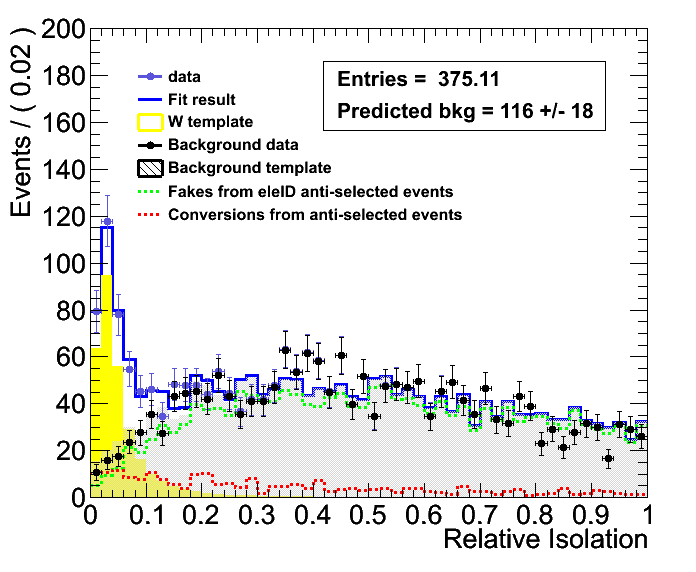
\includegraphics[scale=0.32]{Plots/w_combIso_pt20_fit_MC.png}
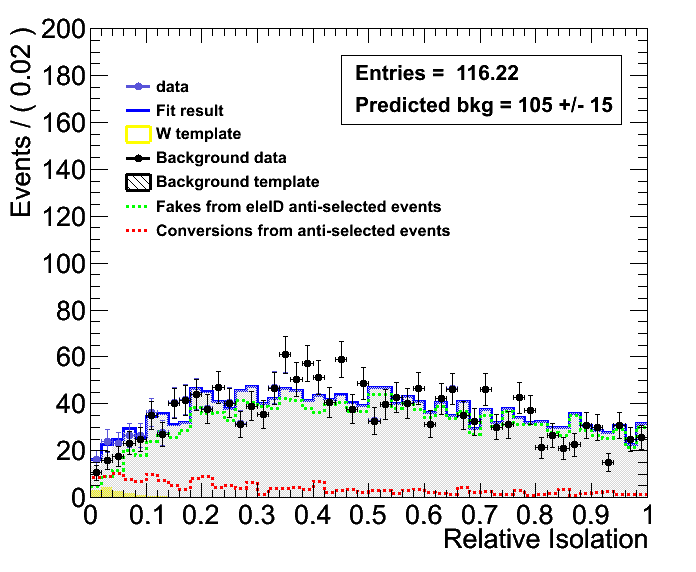
\includegraphics[scale=0.32]{Plots/w_combIso_pt20_METanticut_fit_MC.png}
\caption{\textit{Same as Figure~\ref{fig:w_combIso_fit} only this time for electrons with $P_{T}$ threshold at 20~GeV.  }}\label{fig:w_combIso_fit_pt20}
\end{figure}

\begin{figure}[h!]
\centering
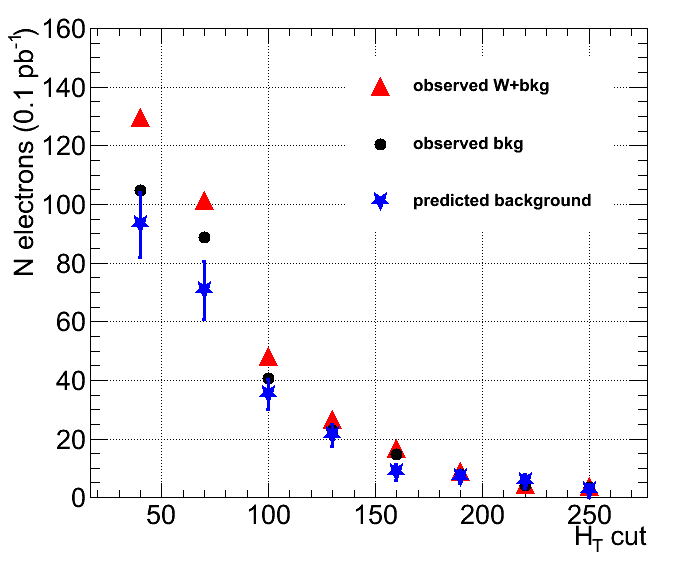
\includegraphics[width=80mm]{Plots/w_fitprediction_pt20_METanticut_vsHT_MC.png}
%\end{center}
%\vspace{1mm}
\caption{\textit{Same as Figure~\ref{fig:w_fitprediction_mc} only this time for electrons with $P_{T}>$ 20~GeV. }}
\label{fig:w_fitprediction_mc_pt20}
\end{figure}


Given the remarkably good description of the combined background in Monte Carlo simulation, we next test this procedure on CMS data.  This is the subject of the next section.

\subsection{Predicting the distribution of the $\alpha{_T}$ kinematic variable by inverting Electron ID Cuts}

Following the promising results of the $\alpha_{T}$ jet-balancing method previously described for the all-hadronic SUSY searches~\cite{njet}, a natural extension of this approach has been developed to the single-lepton SUSY search~\cite{ouratnote}, where a significant presence of QCD multi-jet backgrounds is expected.

The $\alpha_{T}$ variable is here defined as an N-object system where the set of objects is 1 electron and N-1 jets. This definition reproduces the kinematics of a di-jet system by contructing two pseudo-jets, which balance one another in $H_{T}$. The two pseudo-jets are formed from the combination of the N objects that minimizes the $\Delta H_{T} \equiv |H_{T,1} - H_{T,2}|$ of the pseudo-jets, and the resulting  $\alpha_{T}$ is
\begin{equation}
\alpha_{T} = \frac{1}{2} \frac{H_{T} - \Delta H_{T}}{M_{T}} =  \frac{1}{2} \frac{H_{T} - \Delta H_{T}}{\sqrt{H_{T}^{2}-MH_{T}^{2}}}.
\end{equation}

This section is dedicated to a first approach of commissioning the alphaT observable and study its behavior in pure fake electron events. It is therefore desirable to collect a suitable control sample which will be dominated by fake electrons and eliminate sources of prompt electron events (like W events).

One way to obtain such a sample is using the anti-selection method on electron ID variables which are less correlated with the missing transverse energy. In this section, we investigate the possibility of inverting the $\Delta \eta$(trk-SC) and $\Delta \phi$ (trk-SC) id cuts in the electron selection. The selected events in this method pass the pre-selection described in Section~\ref{sec:evtsel}, while the anti-selected are those events which pass the selection with an electron that passes all selection id criteria except the $\Delta \phi$ (trk-SC) and $\Delta \eta$(trk-SC) ones. 

In order to establish the validity of the control sample obtained by the anti-selection method above, the perfomance must be compared of the leptonic $\alpha_T$ as obtained from the control sample and the actual QCD events passing the electron criteria defined in the ``signal'' region. Because SUSY events are expected to have high $H_{T}$, it is desirable to understand how the method evolves with increasing $H_{T}$ cuts. The number of events for 1pb$^{-1}$ passing the pre-selection, and two different cuts in $H_{T}$ are shown for selected in Table \ref{tab:CF_S_20} and for anti-selected in Table \ref{tab:CF_AS_20}. 

\vspace{3mm}
\begin{table}[h!]
\begin{center}
\begin{tabular}{|c||c|c|c|c|c|}
\hline
Cutflow & QCD EM enriched & QCD BC$\rightarrow e$ & QCDJets Pythia $\hat{p_{T}}$ & W & \% contamination from W\\
\hline
\hline
All events & 5351938 & 256514.4 & 25470 & 24170 & 0.43\%\\
N($e^{-}$) $\geq$ 1 & 9372.1 & 2635.5 & 19.9 & 3848.6 & 32\%\\
N($jets$) $\geq$ 1 & 8174.5 & 2317.3 & 10.4 & 3632.48 & 34.6\%\\
HT $>$ 100 GeV & 249.2 & 55.8 & 6.2 & 95.3 & 30.6\%\\
HT $>$ 180 GeV & 7.53 & 1.2 & 3.6 & 2.86 & 23.2\%\\
\hline
\end{tabular}
\end{center}
\caption{\textit{Cutflow for selected events.Numbers shown for 1pb$^{-1}$ for both QCD and W samples used for the anaylsis with electron $p_{T}$ requirement set to 20GeV.}}
\label{tab:CF_S_20}
\end{table}

\begin{table}[h!]
\begin{center}
\begin{tabular}{|c||c|c|c|c|c|}
\hline
Cutflow & QCD EM enriched & QCD BC$\rightarrow e$ & QCDJets Pythia $\hat{p_{T}}$ &  W & \% contamination from W\\
\hline
All events & 5351938 & 256514.4 & 25470 & 24170 & 0.43\%\\
N($e^{-}$) $\geq$ 1 & 32725.5 & 729.0 & 52.9 & 298.0 & 0.89\%\\
N($jets$) $\geq$ 1 & 27545.3 & 609.9 & 28.1 & 271.5 & 0.96\%\\
HT $>$ 100 GeV & 902.8 & 24.9 & 18.3 & 4.9 & 0.52\%\\
HT $>$ 180 GeV & 20.7 & 0.8 & 10.7 & 0.3 & 1.01\%\\
\hline
\end{tabular}
\end{center}
\caption{\textit{Cutflow for anti-selected events.Numbers shown for 1pb$^{-1}$ for both QCD and W samples used for the anaylsis with electron $p_{T}$ requirement set to 20GeV.}}
\label{tab:CF_AS_20}
\end{table}

It can be seen that the anti-selected control sample allows one to study and validate the expected behavior of the $\alpha_{T}$ in a sample of \textit{pure} fake electron events, where the contamination from prompt electrons should be at a level below 1\%, as opposed to the selection region where $W \rightarrow e\nu$ is expected to contribute at the $\approx 10$\% level.

\subsubsection{Closure test with pure QCD background sample}

The control sample provided by anti-selection on the ($\Delta \eta$/$\Delta \phi$) electron id variables must first undergo a closure test with a pure QCD sample. This will show if there is any bias in QCD between the distribution of $\alpha_{T}$ in the selected and the anti-selected regions. The plots in \ref{fig:AlphaTbyHT} show the normalised shape of distributions, firstly before an $H_{T}$ cut (top left) and then as increasing cuts in $H_{T}$ are applied. The selected and anti-selected distributions show good agreement. The evolution of the $\alpha_{T}$ as $H_{T}$ cut increases shows the expected reduction in the tail for $\alpha_{T} >$ 0.55, the region of likely SUSY signal, for both selected and anti-selected events.

\begin{figure}[h!]
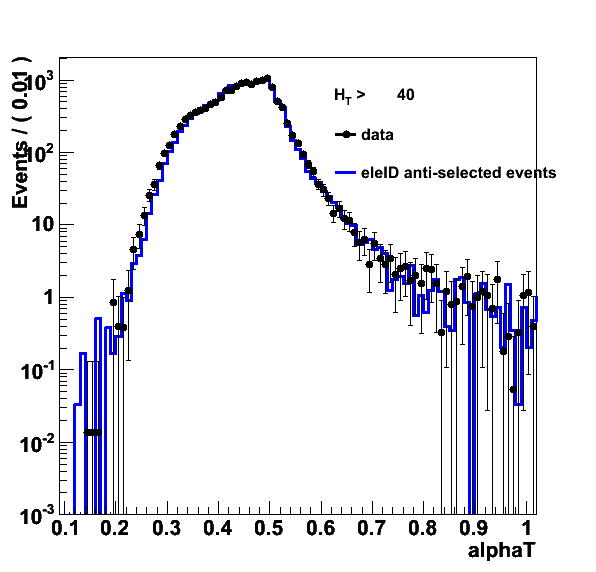
\includegraphics[width=50mm]{Plots/mc-alphaT-1}
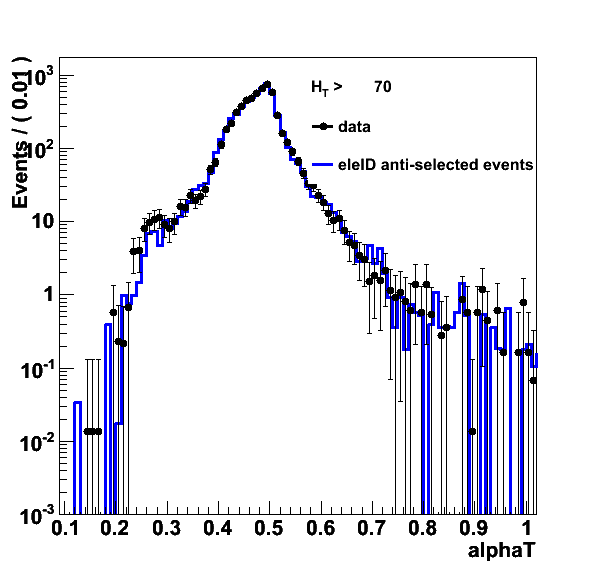
\includegraphics[width=50mm]{Plots/mc-alphaT-2}
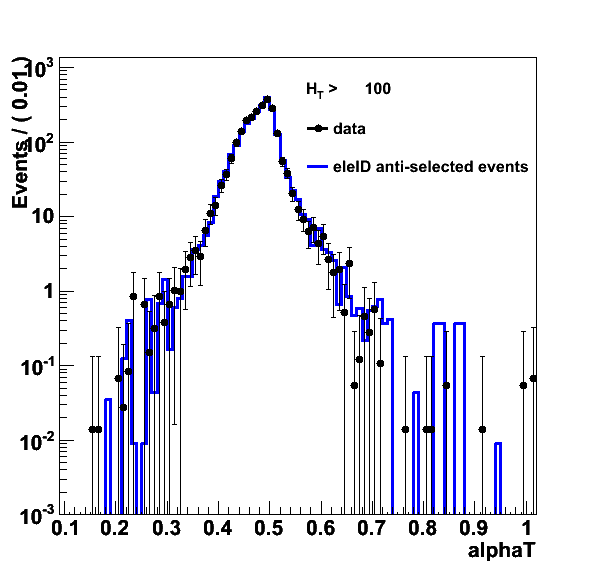
\includegraphics[width=50mm]{Plots/mc-alphaT-3}
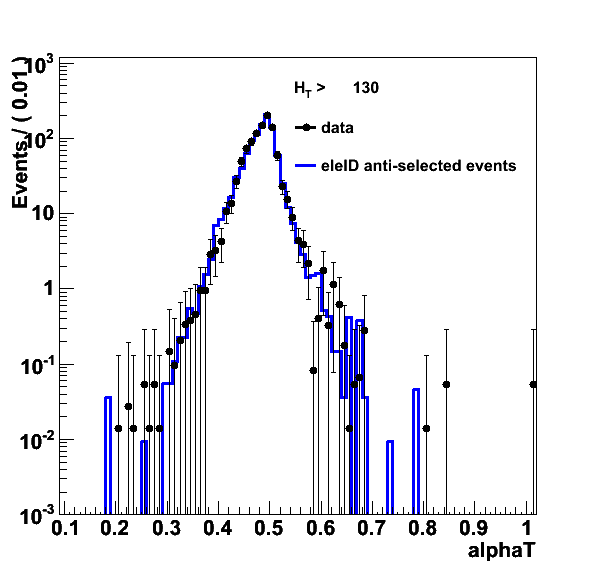
\includegraphics[width=50mm]{Plots/mc-alphaT-4}
\hspace*{3mm}
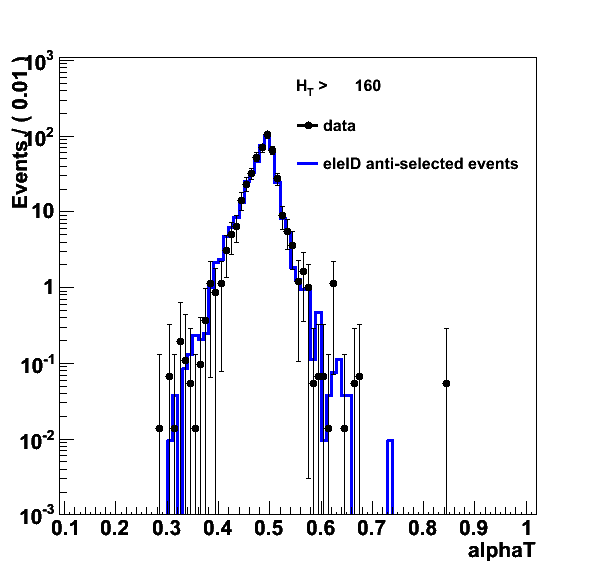
\includegraphics[width=50mm]{Plots/mc-alphaT-5}
\hspace*{3mm}
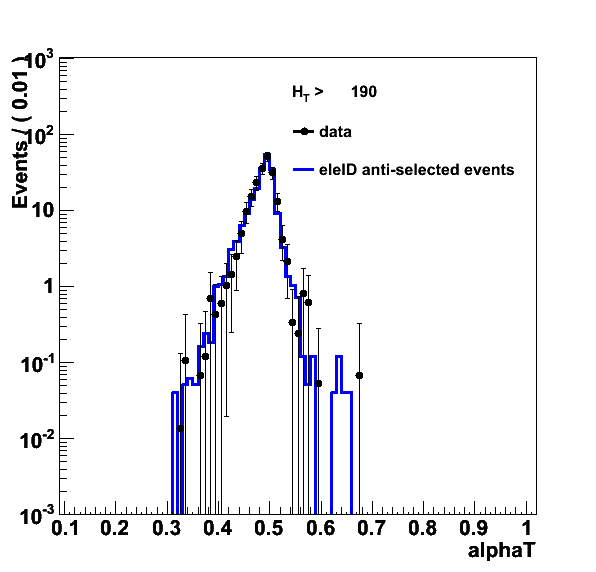
\includegraphics[width=50mm]{Plots/mc-alphaT-6}

\caption{\textit{The $\alpha_{T}$ distributions for selected (red) and anti-selected events (black) for the QCD multi-jet background, from inversion of the $\Delta \phi$ and $\Delta \eta$ ID Cuts, shown without $H_{T}$ cut (Top Left) and with progressive HT cuts (left-right, top-bottom). These distributions are normalised to unity for shape comparison. There is good agreement between the selected and anti-selected samples regardless of HT requirement, and the high $\alpha_{T}$ tails reduce as expected when moving to higher HT cuts.}}
\label{fig:AlphaTbyHT}
\end{figure}

In order to demonstrate the power of $H_{T}$ in $\alpha_{T}$ tail-reduction, we introduce the variable $R_{\alpha_T}$ which is defined as the ratio of the number of events passing the $\alpha_T$ cut over the number of events failing it:
\begin{equation}
R_{\alpha T} = \frac{N(\alpha_{T}>0.55)}{N(\alpha_{T}>0.)}
\end{equation}
The ``default'' cut value here is the value prompted from the all-hadronic analysis, 0.55. Figure \ref{fig:AlphaT_Ratio} shows a plot of $R_{\alpha_T}$ as a function of the $H_{T}$ cut applied. As the $H_{T}$ cut value increases, $R_{\alpha_T}$ is observed to decrease in an (approximately) exponential manner~\cite{david}. This result confirms that the noticable reduction in the tail are much more pronounced than those in the peak, therefore this is not a statistical effect only. The selected and anti-selected events remain in good agreement.

\begin{figure}[h!]
\begin{center}
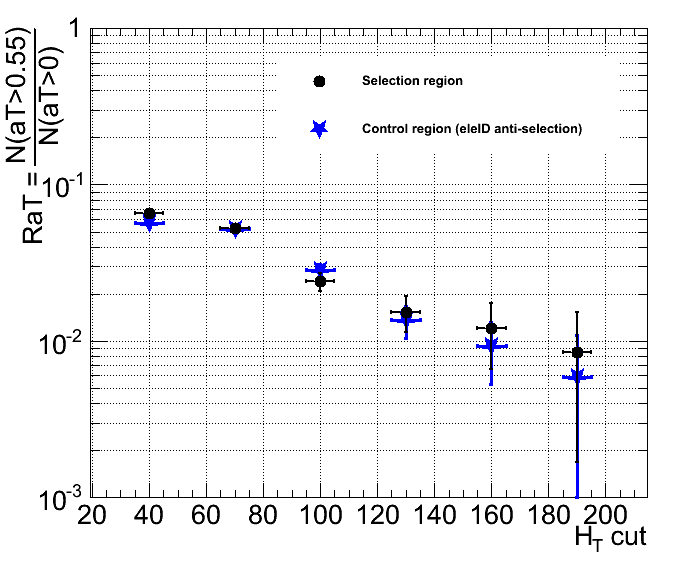
\includegraphics[width=80mm]{Plots/mc-alphaTratio}
\end{center}
\caption{\textit{The $R_{\alpha_T}$ versus the $H_{T}$ cut applied for the QCD multi-jet background, shown for both selected and anti-selected events in the Delta ID Inversion method.}}
\label{fig:AlphaT_Ratio}
\end{figure}

\subsubsection {Closure test with W + jets contamination in control region}

Having acertained the validity of the anti-selection method to predict the QCD contribution in the selected from the QCD in the anti-selected, it is important to test whether the process will work with contamination in the control region. The method is designed for data-driven extimation, and thus must be robust to such contamination.

The closure test is repeated, with the anti-selected now from both the pure QCD sample as before, and W + jets also. The selected remains from pure QCD as a comparison. The normalised ditribution plots shown for this case are in Figure~\ref{fig:w-AlphaTbyHT}, and the plot of $R_{\alpha_T}$ as a function of the $H_{T}$ cut applied is in Figure~\ref{fig:w-AlphaT_Ratio}. 

\begin{figure}[h!]

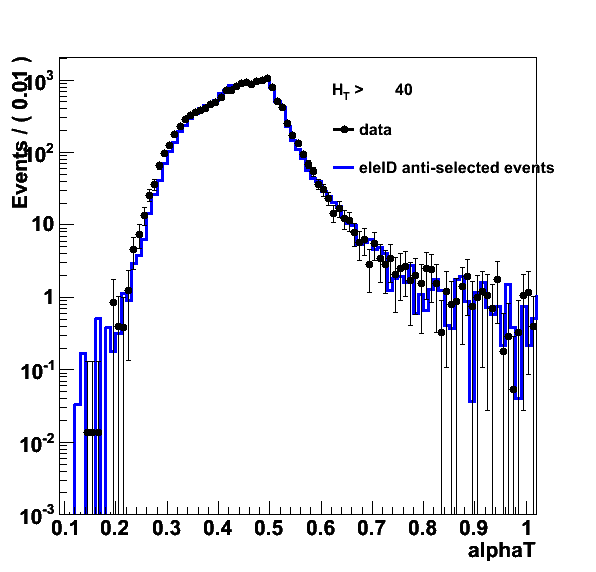
\includegraphics[width=50mm]{Plots/w-alphaT-1}
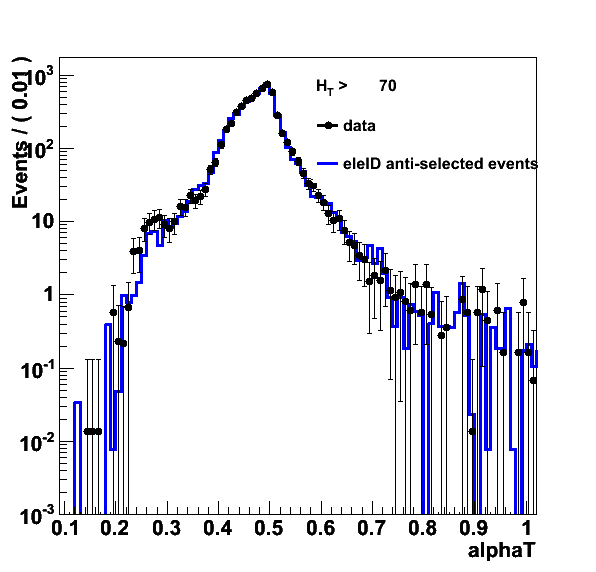
\includegraphics[width=50mm]{Plots/w-alphaT-2}
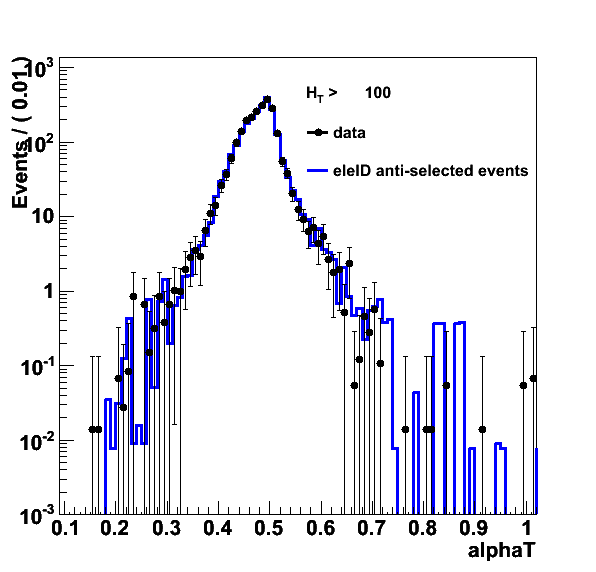
\includegraphics[width=50mm]{Plots/w-alphaT-3}
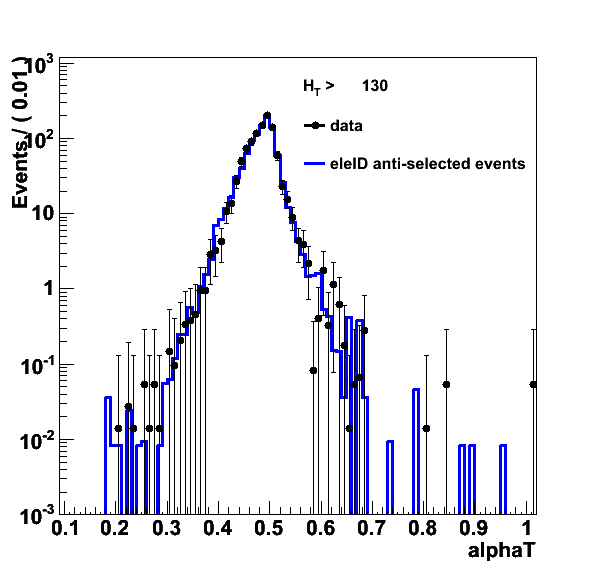
\includegraphics[width=50mm]{Plots/w-alphaT-4}
\hspace*{3mm}
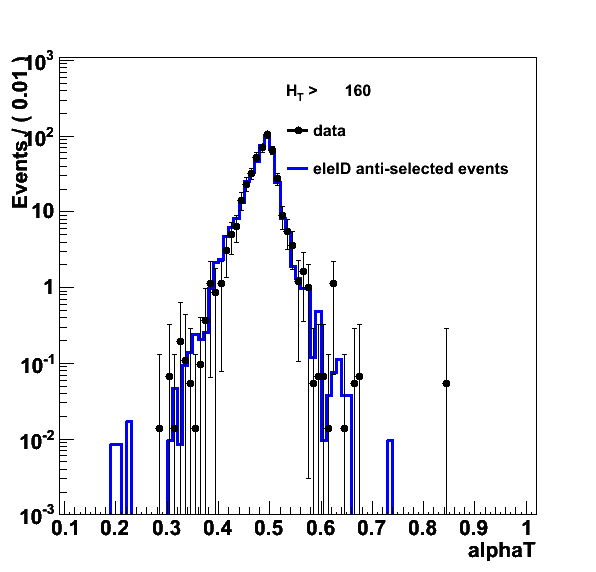
\includegraphics[width=50mm]{Plots/w-alphaT-5}
\hspace*{3mm}
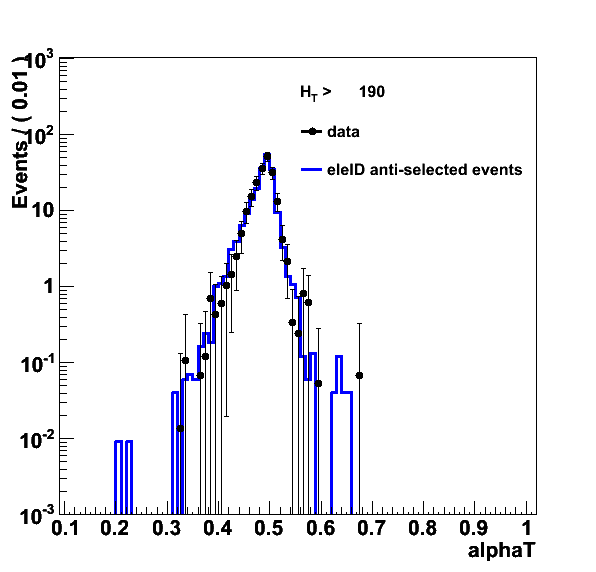
\includegraphics[width=50mm]{Plots/w-alphaT-6}
\caption{\textit{Same as in Figure~\ref{fig:AlphaTbyHT} only this time with W contamination in the control region.}}
\label{fig:w-AlphaTbyHT}
\end{figure}

%Figure \ref{fig:AlphaT_Ratio} shows a plot of $R_{\alpha_T}$ as a function of the $H_{T}$ cut applied. As the $H_{T}$ requirement increases, $R_{\alpha_T}$ decreases in an exponential manner. Thic confirms that the noticable reduction in the tail are much more pronounced than those in the peak, therefore this is not a statistical effect only. The selected and anti-selected events remain in good agreement.

\begin{figure}[h!]
\begin{center}
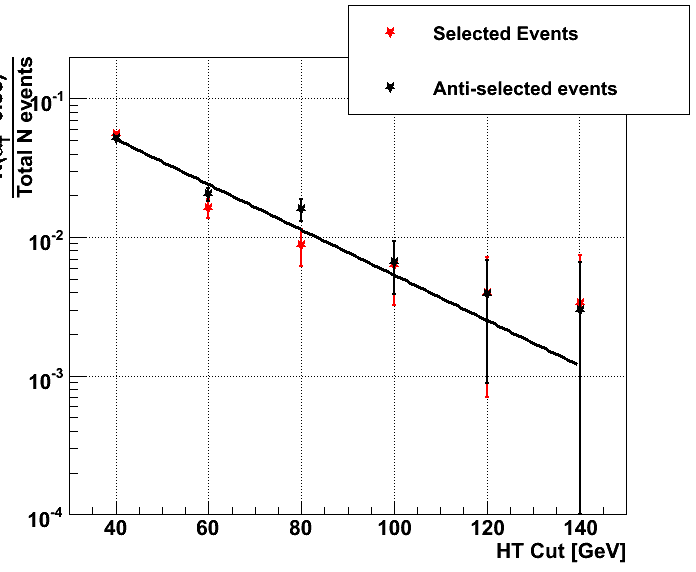
\includegraphics[width=80mm]{Plots/w-alphaTratio}
\end{center}
\caption{\textit{Same as in Figure~\ref{fig:AlphaT_Ratio} only this time with W contamination in the control region.}}
%The $R_{\alpha_T}$ versus the $H_{T}$ cut applied for the QCD multi-jet background, with contamination from W + jets in the anti-selected only, shown for both selected and anti-selected events in the Delta ID Inversion method.}}
\label{fig:w-AlphaT_Ratio}
\end{figure}

Adding in contamination from the W + jets sample has no discernable effect on the shape of the $\alpha_{T}$ distribution, and the ratio remains to good agreement also. The control sample is thus robust to such a contamination, and still remains a good estimator of the shape of the QCD background for the selected events.

\begin{comment}
\subsubsection{Closure test with lowered electron $P_{T}$ threshold}
It is also important to commission $\alpha_{T}$ as the electron $p_{T}$ requirement is lowered. The study is repeated with the electron $p_{T} >$ 10 GeV. Tables \ref{tab:CF_S_10} and \ref{tab:CF_AS_10} show the numbers for selected and anti-selected cutflows respectively at $1pb^{-1}$. 

\begin{table}[h!]
\begin{center}
\begin{tabular}{|c||c|c|c|c|}
\hline
Cutflow & QCD EM enriched & QCD BC$\rightarrow e$ & QCDJets Pythia $\hat{p_{T}}$ &  W \\
\hline
All events & 5351938 & 256514.4 & 25470 & 17830 \\

N($e^{-}$) $\geq$ 1 & 22120.98 & 13117.37 & 4.37 & 2953.69\\

N($jets$) $\geq$ 1 & 14783.29 & 7811.25 & 4.37 & 761.22\\

HT $>$ 100 GeV & 846.64 & 312.95 & 4.37 & 78.73\\

HT $>$ 180 GeV & 159.83& 36.05 & 4.29 & 18.20\\
\hline
\end{tabular}
\end{center}
\caption{\textit{Cutflow for selected events.Numbers shown for 1pb$^{-1}$ for both QCD and W samples used for the anaylsis with electron $p_{T}$ requirement set to 10GeV.}}
\label{tab:CF_S_10}
\end{table}

\begin{table}[h!]
\begin{center}
\begin{tabular}{|c||c|c|c|c|}
\hline
Cutflow & QCD EM enriched & QCD BC$\rightarrow e$ & QCDJets Pythia $\hat{p_{T}}$ &  W \\
\hline
All events & 5351938 & 256514.4 & 25470 & 17830\\
N($e^{-}$) $\geq$ 1 & 44807.39 & 1406.28 & 3.30 & 173.04\\
N($jets$) $\geq$ 1 & 30089.89 & 920.40 & 3.30 & 43.52\\
HT $>$ 100 GeV & 1291.41 & 51.64 & 3.29 & 4.05\\
HT $>$ 180 GeV & 112.68 & 5.55 & 3.20 &  0.92\\
\hline
\end{tabular}
\end{center}
\caption{\textit{Cutflow for anti-selected events.Numbers shown for 1pb$^{-1}$ for both QCD and W samples used for the anaylsis with electron $p_{T}$ requirement set to 10GeV.}}
\label{tab:CF_AS_10}
\end{table}

\end{comment}


%\clearpage

%\newpage
\section{Commissioning Background Estimation Methods with 7TeV Data}

Having shown that the two background estimation methods work well in Monte Carlo simulation, we next take a look at the results using collision data, and, for comparison a Monte Carlo sample generated by PYTHIA8 to be non process-specific. 

It is intentional for this analysis to commission low-$p_{T}$ electrons (of offline thresholds below the standard online threshold of the single electron trigger); and therefore the data sample is chosen from the JetMETTau secondary datasets, which are subject to JetMET triggers. The data sample used in this study is taken from the Secondary Dataset (SD) JetMETTau, and the HLT trigger applied on top of the selection is the HLT\_Jet15U.

The 7TeV collision data used to demostrate the performance of the Background Estimation methods described in this Note, amounts to 12.47 $\text{nb}^{-1}$ of integrated luminosity.

\subsection{Commissioning the Isolation Template method with first data}

The data are selected as described in section~\ref{sec:evtsel}. Events with at least one electron with $p_{T}>$ 10 GeV and passing all standard electron identification, as well with a minimal hadronic activity of $H_{T} >$ 20 GeV - equivalent to the requirement of at least one jet with $p_{T}>$ 20 GeV -, are used to plot the combined Isolation distribution in the Selection region. A three-template fit is used to model the Isolation distribution in the Selection region, with two-template background component taken from the two control regions which defined earlier, and a single W-component to describe the $W \rightarrow e\nu$ shape. The W-shape is used here directly from a MC template ($We\nu$ PYTHIA sample) in order to test the Isolation template method.  

Figures~\ref{fig:d_combIso_fit} show the full fit to the Isolation distribution in the Selection region, with the right plot repeating the exercise with a $pfMET < 20$~GeV cut. In both cases there is a good agreement between the Isolation shape selected and the modeling distributions extracted from the control regions. A first evidence of W-signal contamination is apparent on the plots; with the left one showing an excess of events from the predicted background, and the right one showing the suppression of the signal using the pfMET ``anti-cut''. 

Since, as was shown in section~\ref{sec:modeling}, we observed a small deviation between the Calorimeter Isolation distributions in the Control and Selection Regions (prior to re-weighting as described above) we would like to confirm that the good description of the full Isolation distribution, i.e. with all backgrounds combined, remains good for different regions in the overall hadronic selection of the events.  For this reason, we repeat the fits for different values of the total $\text{H}_{T}$ of the event.  The fits yield a number of expected events passing the RelIso$<0.3$ requirement -- and this number can be compared to the actual number seen in the data.  We summarize these results in Figure~\ref{fig:d_fitprediction} where a very good agreement between the predicted and observed event yields is seen.


\begin{figure}[h!]
\centering
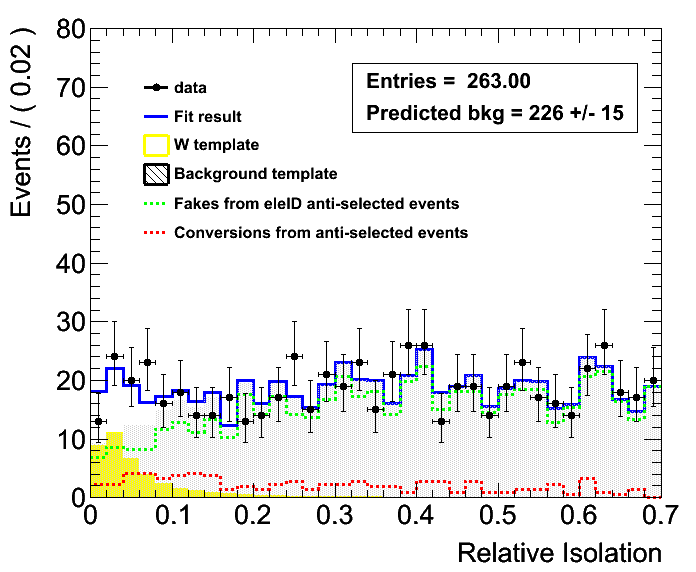
\includegraphics[scale=0.32]{Plots/d_combIso_pt10_fit.png}
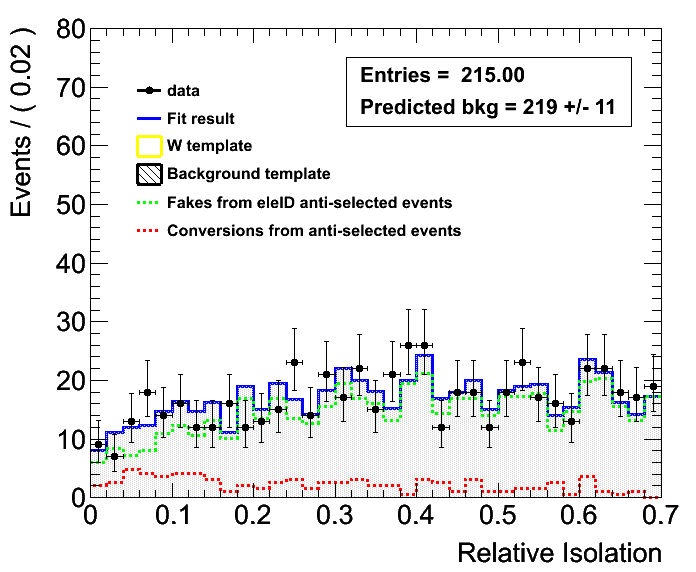
\includegraphics[scale=0.32]{Plots/d_combIso_pt10_METanticut_fit.png}
\caption{\textit{The combined Isolation distribution for 10 GeV electrons in data (points) and its breakdown into three components, one for the combined background from jets and heavy-flavors (Jet-e and HF-e), another for conversions (Conv-e) and a third for the W $\rightarrow e\nu$. The dashed lines are the two background components as extracted from the two Control Samples, whereas the sum of the ``predicted'' background is shown in filled grey. On the right plot, a pfMET $ < 20$~GeV anti-cut has been applied.  }}
\label{fig:d_combIso_fit}
\end{figure}

\begin{figure}[h!]
\centering
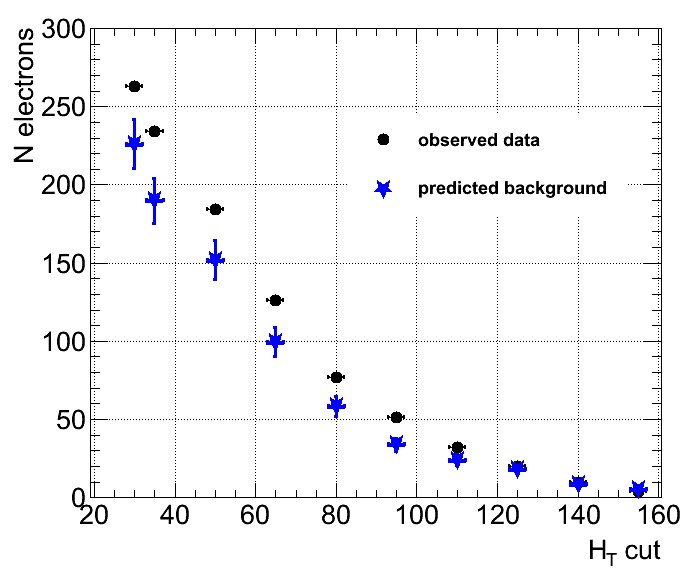
\includegraphics[scale=0.32]{Plots/d_fitprediction_pt10_vsHT.png}
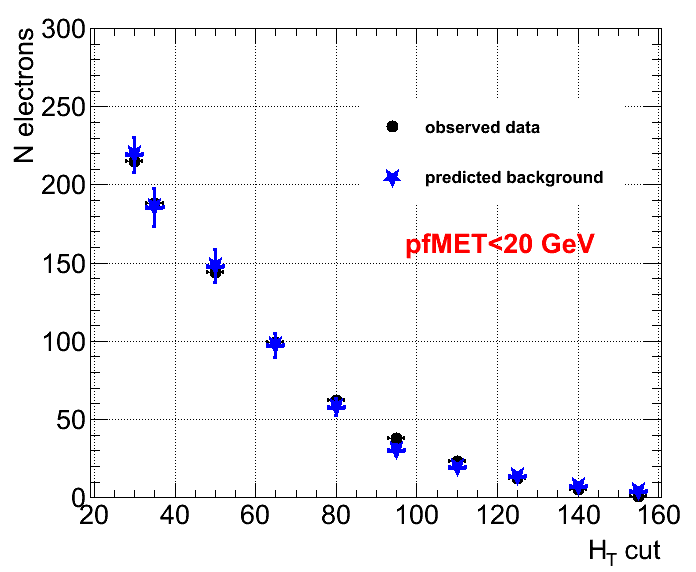
\includegraphics[scale=0.32]{Plots/d_fitprediction_pt10_METanticut_vsHT.png}
%\end{center}
\caption{\textit{The observed number of electrons (in black dots) in signal region, RelIso $< 0.3$, are compared to the fit prediction (in blue stars), as a function of the cut in the hadronic activity of the event ($H_{T}$ cut). A pfMET anti-cut at 20~GeV has been applied to suppress sources of prompt electrons (e.g. Ws). }}
\label{fig:d_fitprediction}
\end{figure}

%The same procedure is applied to events with electrons with $p_{T} >$ 20 GeV, and the result can be in inspected similarly on Figures~\ref{fig:d_combIso_fit_pt20} and~\ref{fig:d_fitprediction_pt20}. The evidence of the W component present in the selection is now more prominent with the level of background being significantly lower with respect to the $p_{T}(e)>10 $ GeV case. The overall results show a compatible behavior with the corresponding MC results presented in section~\ref{mc_wcontamin}. 


\begin{figure}[h!]
\centering
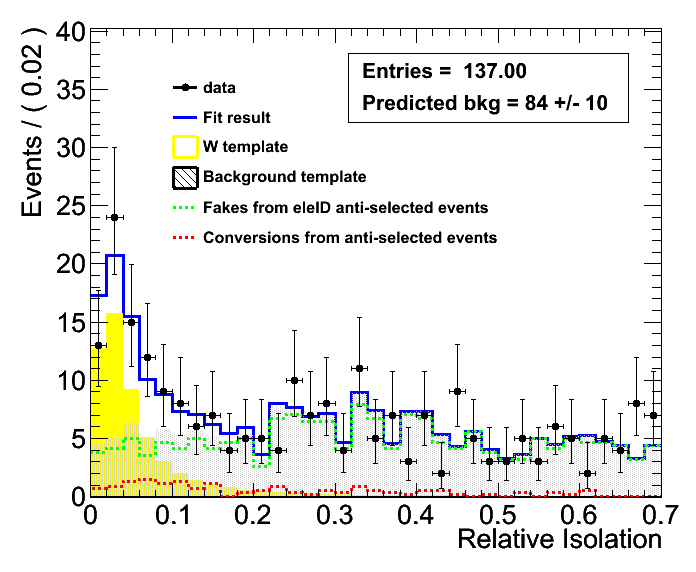
\includegraphics[scale=0.32]{Plots/d_combIso_pt20_fit.png}
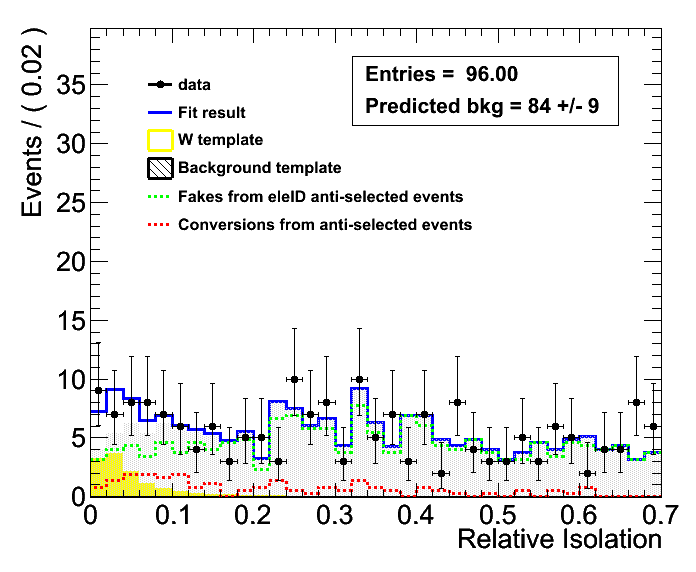
\includegraphics[scale=0.32]{Plots/d_combIso_pt20_METanticut_fit.png}
\caption{\textit{Same as Figure~\ref{fig:d_combIso_fit} only this time for electrons with $P_{T}$ threshold at 20 GeV.  }}
\label{fig:d_combIso_fit_pt20}
\end{figure}

\begin{figure}[h!]
\centering
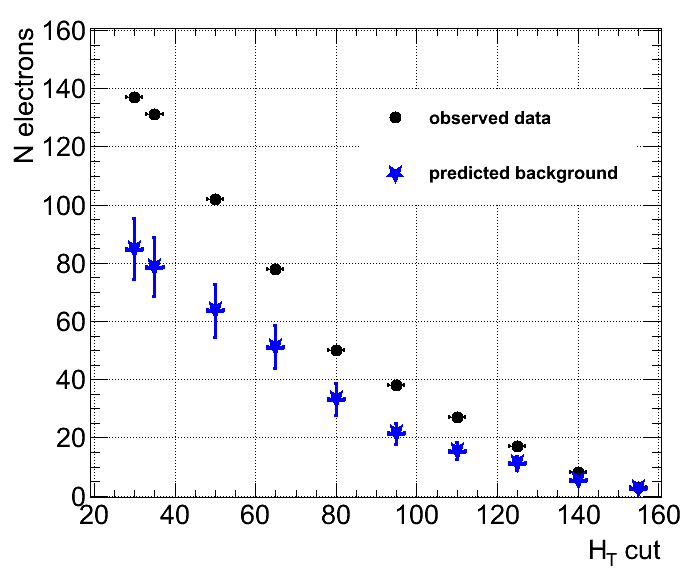
\includegraphics[scale=0.32]{Plots/d_fitprediction_pt20_vsHT.png}
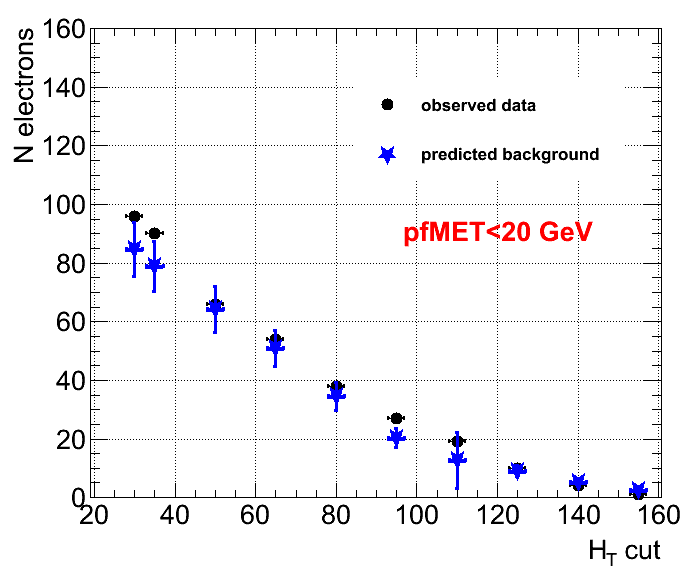
\includegraphics[scale=0.32]{Plots/d_fitprediction_pt20_METanticut_vsHT.png}
%\end{center}
\caption{\textit{Same as Figure~\ref{fig:d_fitprediction} only this time for electrons with $P_{T}$ threshold at 20 GeV. }}
\label{fig:d_fitprediction_pt20}
\end{figure}

The same procedure is applied to events with electrons with $p_{T} >$ 20 GeV, and the result can be in inspected similarly on Figures~\ref{fig:d_combIso_fit_pt20} and~\ref{fig:d_fitprediction_pt20}. The evidence of the W component present in the selection is now more prominent with the level of background being significantly lower with respect to the $p_{T}(e)>10 $ GeV case. The overall results show a compatible behavior with the corresponding MC results presented in section~\ref{mc_wcontamin}.

%The fits also yield a number of expected events passing the RelIso$<0.3$ requirement -- and this number can be compared to the actual number seen in the data.  We summarize these results in Table~\ref{tab:IsoFits} where a very good agreement between the predicted and observed event yields is seen.  

\begin{comment}
\begin{table}[h!]
\vspace{5mm}
\begin{center}
\begin{tabular}{|c||c|c||c|c|}
\hline
&\multicolumn{2}{c|}{$p_{T}(e) > 5 \text{GeV}$}&\multicolumn{2}{c|}{$p_{T}(e) > 10 \text{GeV}$}\\
\cline{2-5}
& \textbf{Observed} & \textbf{Predicted} & \textbf{Observed} &  \textbf{Predicted} \\
\hline
\hline
$H_{T}>20 \text{GeV}$ & $115.$ & $115.4 \pm 7.5$ & $98.$ & $99.6 \pm 7.4$ \\
$H_{T}>40 \text{GeV}$ & $54.$ & $56.5 \pm 5.3$ & $46.$ & $48.9 \pm 5.0$ \\
$H_{T}>60 \text{GeV}$ & $31.$ & $31.8 \pm 2.6$ & $24.$ & $25.6 \pm 2.4$ \\
\hline
\end{tabular}
\end{center}
\caption{\textit{Summary of fit results predicting the number of electrons that fall in the calorimeter Isolation region of CaloIso$<0.1$, using the two-template fit. The data sample is taken from the SD JetMETTau of the 7TeV collision data, using the trigger HLT\_Jet15U. }}
\label{tab:IsoFits}
\end{table}
\vspace{5mm}
\end{comment}

The results obtained using the data-driven control samples are quite encouraging that these samples may also be used to obtain the shapes observed in data for more intricate topological variables.  This is the subject of the following section.

\subsection{Commissioning the cut-based electron ID Inversion method with first data}

Due to the limited statistics collected so far, currently the selection is loosened in the following ways:
\begin{itemize}
\item The electron offline $p_{T}$ threshold is lowered to 10 GeV.
\item The electronID is applied according to the official recommendations of the CMS Egamma POG. The electron isolation is chosen to be the Relative Calorimeter Isolation, with the value of the cut loosened to 0.3.
\item At least one jet with $p_{T} > 40$~GeV corrected transverse energy.
\item The $H_{T}$ cuts applied are lowered to study the evolution without losing all valid statistics.
\end{itemize}

Because SUSY events are expected to appear in high $H_{T}$ regimes, we examine the behaviour of the $\alpha_{T}$ distribution as a function of $H_{T}$. Figure~\ref{fig:datamc} show the $\alpha_{T}$ distributions for selected and anti-selected events from collision data, in succesive cuts in $H_{T}$, whereas a $pfMET < 20$ GeV cut has been applied. The selected and anti-selected distributions show a good agreement. However, the selected distributions are susceptible to W contamination at higher level than the anti-selected ones. 

To measure the reduction in high aT events, we plot the ratio $ RaT  = N(aT>0.55)/ N(aT>0) $ as a function of the $H_{T}$ cut in Fig.~\ref{fig:datamcRat}. $RaT$ does show an approximately exponential decrease with $H_{T}$, a performance which can be reliably validated using the anti-selected events. 

\begin{figure}[h!]

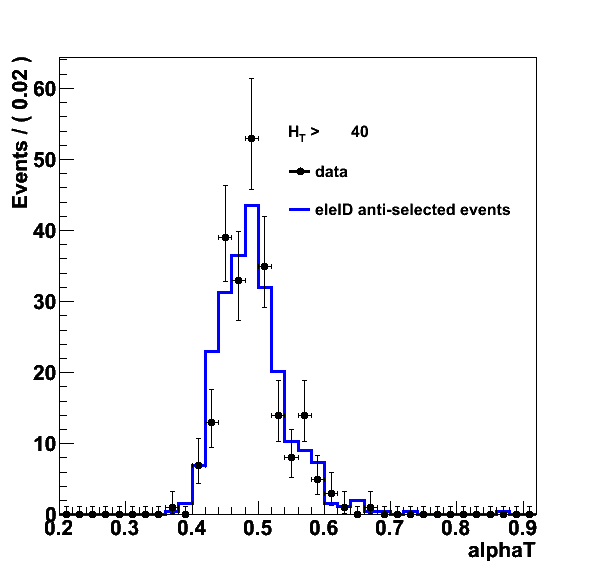
\includegraphics[width=50mm]{Plots/d-alphaT-1}
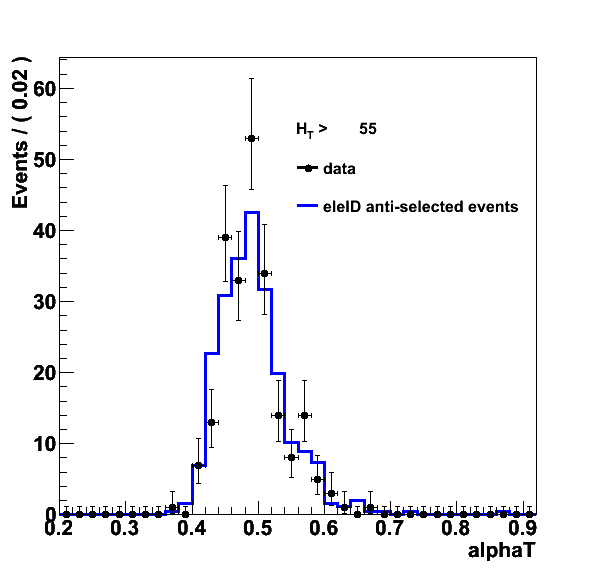
\includegraphics[width=50mm]{Plots/d-alphaT-2}
\includegraphics[width=50mm]{Plots/d-alphaT-3}
\includegraphics[width=50mm]{Plots/d-alphaT-4}
\hspace*{3mm}
\includegraphics[width=50mm]{Plots/d-alphaT-5}
\hspace*{3mm}
\includegraphics[width=50mm]{Plots/d-alphaT-6}
\caption{\textit{The $\alpha_{T}$ distributions for selected (red) and anti-selected events (black) from collision data shown with progressive cuts in $H_{T}$. These distributions are normalised to each other for shape comparison. There is good agreement between the selected and anti-selected samples regardless of $H_{T}$ requirement, and the high $\alpha_{T}$ tails are reduced as expected when moving to higher $H_{T}$ cuts.}}
\label{fig:datamc}
\end{figure}
%\hspace*{3mm}
\begin{figure}[h!]
\centering
\includegraphics[scale=0.32]{Plots/RaT_pt10.png}
\includegraphics[scale=0.32]{Plots/RaT_pt10_anticut.png}
%\hspace*{13mm}
%\includegraphics[width=80mm]{Plots/RaT_pt10_anticut_MCP8.png}
\caption{\textit{The $R_{\alpha_T}$ versus the $H_{T}$ cut applied for collision data, shown for both selected and anti-selected events in the ID Inversion method. The right plot includes a cut at pfMET$<20$~GeV to eliminate contamination of prompt electron sources (e.g. Ws). The collision data amounts to 12.47 nb$^{-1}$.}}
\label{fig:datamcRat}
\end{figure}


\section{Summary}
\label{sec:Summary}

This study proposes two methods of data-driven QCD background estimation, and presents results from Monte Carlo and the first X pb$^{-1}$ of 7TeV data taken by CMS at the LHC. 

Following the promising results of studies into using the $\alpha_{T}$  kinematic variable in the single electron mode of SUSY searches, it is proposed that a suitable control sample in the distribution of this variable for predicting the QCD background could be obtained by inverting the $\Delta \phi$ and $\Delta \eta$ cuts in the electron selection criteria. 

The analysis uses Monte Carlo samples to perform a closure test on this method, first with a pure QCD sample, and then with W + jets contamination in the anti-selected control sample. The method proved unbiased between selected and anti-selected in these tests. 

The first look at this method under 7TeV collision data and corresponding Monte Carlo is also shown, with lowered selection to maximise available statistics.

\clearpage

\begin{thebibliography}{9}
%\bibitem{lisa}{L.~Randall and D.~Tucker-Smith, {\em``Dijet searches for Supersymmetry at the LHC''}, Phys. Rev. Lett. \bf{101} (2008) 221803, arXiv:0806.1049.}
\bibitem{data}{https://twiki.cern.ch/twiki/bin/view/CMS/ProductionSummer2009.}
\bibitem{mad}{J~Alwall et al., ``MadGraph/MadEvent v4: The New Web generation'', JHEP 09 (2007) 028, arXiv:0706.2334.}
\bibitem{susypat1} {https://twiki.cern.ch/twiki/bin/view/CMS/SusyPat.}
\bibitem{susypat2} {https://twiki.cern.ch/twiki/bin/view/CMS/SWGuidePAT.}
\bibitem{susypat}{https://twiki.cern.ch/twiki/bin/view/CMS/SusyPatLayer1.}
\bibitem{ICNT}{https://twiki.cern.ch/twiki/bin/view/CMS/SusyCAFNtupleV000804XX.}
\bibitem{PDWG}{https://twiki.cern.ch/twiki/bin/view/CMS/PhysicsSecondaryDatasets.}
\bibitem{elsel}{https://twiki.cern.ch/twiki/bin/view/CMS/SimpleCutBasedEleID.}
\bibitem{conv}{https://twiki.cern.ch/twiki/bin/view/CMS/ConversionBackgroundRejection.}
\bibitem{cornel}{L.~Agostino, A.~Chatterjee, R.~Patterson, D.~Puigh, W.~Sun, J.~Thom, J.~Vaughan, P.~Wittich, ``Estimation of Fake Electron background using Data-Driven Techniques'', CMS Analysis Note 2010/043.}
\bibitem{elecid}{J.~Branson, M.~Gallinaro, P.~Ribeiro, R.~Salerno, M.~Sani, ```A cut based method for electron identification in CMS'', CMS Analysis Note 2008/082.}
\bibitem{njet}{H.~Flaecher, M.~Stoye, T.~Rommerskirchen, T.~Yetkin, T.~Whyntie, R.~Bainbridge, J.~Marrouche, {\em``Search for SUSY with exclusive n-jet events''}, CMS Analysis Note 2008/082. }
\bibitem{ouratnote}{O.~Buchmueller, L.~Gouskos, Z.~Hatherell, G.~Karapostoli, A.~Sparrow, P.~Sphicas, ``An application of the $\alpha_{T}$ jet-balancing method to the single-lepton mode SUSY searches,'' CMS Analysis Note 2009/188.}
\bibitem{david}{Paul Geffert and David Stuart, ``Study of the Correlation between $\alpha_{T}$ and $H_{T}$ using Z+jets events'', CMS Analysis Note 2009/155.}



\end{thebibliography}

\end{document}
